% =============================================================================
% DPS-LLM paper, TMLR version. The text is shared with the ACL version:
% edit body.tex and appendix.tex, not this file.
% Build: pdflatex paper_tmlr && bibtex paper_tmlr && pdflatex paper_tmlr && pdflatex paper_tmlr
% [preprint] shows authors; omit the option for anonymous review.
% =============================================================================
\documentclass{article}
\usepackage[preprint]{tmlr}
\usepackage{hyperref}
\usepackage{url}
\usepackage{amsmath}
\usepackage{amssymb}
\usepackage{amsthm}
\usepackage{booktabs}
\usepackage{graphicx}
\usepackage{microtype}
\usepackage{array}
\usepackage{adjustbox}
\newtheorem{theorem}{Theorem}
\newtheorem{proposition}{Proposition}
% single-column layout: keep column-width figures at a readable size
\newcommand{\figwidth}{0.62\textwidth}
\newcommand{\repourl}{\url{https://github.com/mirfan899/parameter-splitting-llm}}

\title{Function-Preserving Width Splitting of Pre-trained LLMs: Exact Expansion, a Hidden Learning-Rate Change, and the Limits of Symmetry-Breaking Noise}

\author{\name Muhammad Irfan \email mirfan.mscs15seecs@seecs.edu.pk \\
\addr School of Electrical Engineering and Computer Science (SEECS)\\
National University of Sciences and Technology (NUST), Islamabad, Pakistan
\AND
\name M. Ali Tahir \email ali.tahir@seecs.edu.pk \\
\addr School of Electrical Engineering and Computer Science (SEECS)\\
National University of Sciences and Technology (NUST), Islamabad, Pakistan}

\begin{document}
\maketitle

% Shared text of the paper, \input by every venue file (paper_acl.tex for ARR and arXiv,
% paper_icml.tex, paper_ijcai.tex, paper_colm.tex, paper_tmlr.tex). Edit the paper here.
% A venue file may predefine these before % Shared text of the paper, \input by every venue file (paper_acl.tex for ARR and arXiv,
% paper_icml.tex, paper_ijcai.tex, paper_colm.tex, paper_tmlr.tex). Edit the paper here.
% A venue file may predefine these before % Shared text of the paper, \input by every venue file (paper_acl.tex for ARR and arXiv,
% paper_icml.tex, paper_ijcai.tex, paper_colm.tex, paper_tmlr.tex). Edit the paper here.
% A venue file may predefine these before \input{body}:
\providecommand{\figwidth}{\columnwidth}          % width of single-column figures
\providecommand{\appref}[1]{Appendix~\ref{#1}}   % IJCAI: appendix is supplementary
\providecommand{\ethicsheading}{Ethics Statement} % ICML: Impact Statement

\begin{abstract}
Growing a pre-trained large language model (LLM) in place, instead of training a larger one from scratch, needs an expansion that preserves the model's function and a way to make the added parameters useful.
We study \textbf{Discriminative Parameter Splitting for LLMs (DPS-LLM)}, which doubles the intermediate width of every SwiGLU feed-forward block by duplicating the gate and up projections and the $\tfrac{1}{2}$-scaled down projection, and breaks the symmetry of the copies with a polarity-preserving, anti-symmetric perturbation adapted from LSTM acoustic models.
We prove that the split is exactly function-preserving and that the anti-symmetric pairing cancels first-order output drift, and confirm both on eight open-weight models from 360M to 1.7B parameters: in float32, the DPS split changes validation perplexity by at most $1.3\times10^{-6}$, two orders of magnitude less than Gaussian noise of the same size.
Its effect on fine-tuning is not what growth methods assume. We prove that under Adam an exact split trains like its seed with a doubled learning rate on the down projection, and a matched control, the unexpanded model with that learning rate, reproduces the split's perplexity reduction on every model and dataset, within $0.18$ points in 15 of 18 settings and within seed noise in the other three.
The perturbation does not break the symmetry: in float32 the distance between paired neurons stays constant during fine-tuning, and DPS-LLM, Gaussian noise and exact duplication are statistically indistinguishable. At each model's best learning rate, the split model, 54--75\% larger, is ahead of its seed on only three of nine settings.
We release code, notebooks and all per-seed results, and argue that evaluations of model growth need matched learning-rate controls.
\end{abstract}

% -----------------------------------------------------------------------------
\section{Introduction}
Transformer LLMs \citep{vaswani2017attention,touvron2023llama,qwen2024technical} are almost always trained under a \emph{static} paradigm: every dimension of the network is fixed \textit{a priori}, the weights are drawn from a random initialization \citep{glorot2010understanding,he2015delving}, and the model is trained end-to-end.
Scaling laws \citep{kaplan2020scaling,hoffmann2022chinchilla} make the cost of this paradigm explicit: a larger model must be trained from scratch, spending much of its early budget on features a smaller model already possesses.
The same rigidity appears at fine-tuning time. When a compact model saturates its parametric capacity on a domain-specific task, practitioners must either accept the plateau or restart with a larger architecture.

Progressive growth offers an alternative: begin with a compact \emph{seed} model and enlarge it during training \citep{chen2015net2net,gong2019stacking,chen2022bert2bert,wang2023ligo}.
Two requirements make growth practical for modern LLMs.
First, the expansion must be \emph{function-preserving}, so that the grown model neither loses the seed's knowledge nor suffers a loss spike.
Second, the duplicated parameters must be \emph{distinguishable}; otherwise identical copies receive identical gradients and the added capacity is never used \citep{chen2015net2net}.
Existing work on Transformers has addressed these requirements for pre-LayerNorm blocks with ReLU or GELU feed-forward layers \citep{chen2022bert2bert,wang2024lemon}, but gated SwiGLU blocks \citep{shazeer2020glu}, which are now standard in LLaMA, Mistral, Gemma, Qwen and SmolLM, multiply two projections element-wise, so naive duplication doubles the block's output.

We adapt \emph{Discriminative Parameter Splitting} \citep{irfan2021discriminative}, originally developed for growing LSTM acoustic models, to SwiGLU Transformers, and ask whether it delivers on both requirements when a pre-trained LLM is fine-tuned. Our contributions are:
\begin{itemize}
    \item \textbf{An exact function-preserving SwiGLU split with drift-cancelling noise.} Duplicating the rows of $W_{gate}$ and $W_{up}$ and the columns of $\tfrac{1}{2}W_{down}$ doubles $d_{ffn}$ with provably identical output (Theorem~\ref{thm:invariance}), and a polarity-signed, anti-symmetric perturbation cancels first-order drift (Proposition~\ref{prop:drift}). Both hold on real checkpoints.
    \item \textbf{A split is a learning-rate change.} Under Adam, an exact split trains like its seed with a doubled learning rate on $W_{down}$ (Proposition~\ref{prop:lr}). We introduce the matched control this implies and show that it reproduces the split's gains.
    \item \textbf{A controlled benchmark.} On eight open-weight models from four families (360M--1.7B), two datasets, five conditions, three seeds, per-model learning-rate sweeps and ablations, we find no gain from added capacity and no symmetry breaking during fine-tuning.
    \item \textbf{A precision pitfall.} In bfloat16 the default perturbation is rounded away entirely; we give a stochastic-rounding protocol under which it survives.
\end{itemize}
We also describe, and release code for, two further regimes of the same operator---dense-to-Mixture-of-Experts (MoE) upcycling and LoRA rank doubling---which we leave for empirical evaluation in future work (\appref{app:regimes}).

\begin{figure}[t]
    \centering
    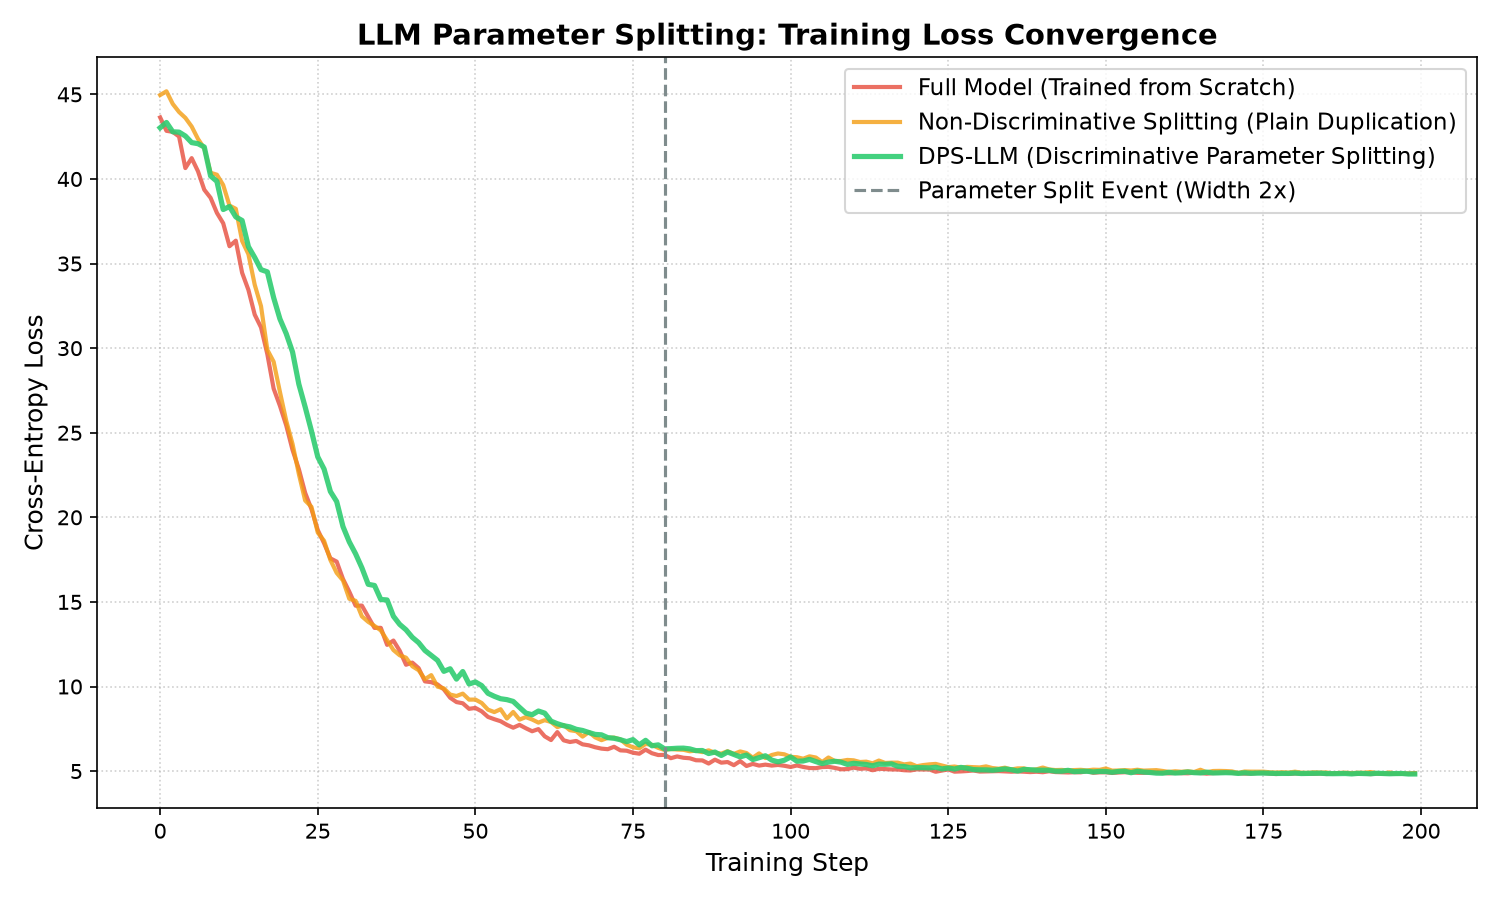
\includegraphics[width=\figwidth]{dps_llm_training_curve.png}
    \caption{\textbf{Controlled split on a synthetic language-modelling task.} A two-layer SwiGLU Transformer with $d_{ffn}=64$ is trained for 80 steps and then split to $d_{ffn}=128$ (dashed line). Both split variants continue without a loss spike, whereas the $d_{ffn}=128$ model trained from scratch spends its first 80 steps re-learning what the seed already knows. DPS-LLM and plain duplication converge to the same loss as the full model by step 200.}
    \label{fig:training_curve}
\end{figure}

% -----------------------------------------------------------------------------
\section{Related Work}
\paragraph{Function-preserving growth.}
Net2Net \citep{chen2015net2net} introduced \emph{Net2WiderNet} and \emph{Net2DeeperNet}, which widen or deepen a network without changing its function, and noted that a small amount of noise is needed to break the symmetry of copied units. Network morphism \citep{wei2016morphism} generalised the idea to arbitrary non-linear morphisms.
For Transformers, progressive stacking \citep{gong2019stacking} and staged training \citep{shen2022staged} grow depth and width of BERT-style encoders; bert2BERT \citep{chen2022bert2bert} extends Net2Net to attention blocks with function-preserving and advanced knowledge initialisation; LiGO \citep{wang2023ligo} learns a linear growth operator from the small model; MSG \citep{yao2024msg} and LEMON \citep{wang2024lemon} obtain lossless expansion for pre-LayerNorm blocks by masking or by an explicit average-and-cancel construction.
Depth up-scaling \citep{kim2024solar} and HyperCloning \citep{samragh2024hypercloning} apply the same principle to decoder-only LLMs, the latter by tiling weights of a small model into a wider one.
DPS-LLM belongs to this family but targets the gated SwiGLU block specifically, where the $\tfrac{1}{2}$ factor must be placed on the down projection to preserve function.

\paragraph{Neuron splitting.}
Splitting steepest descent \citep{liu2019splitting}, Firefly descent \citep{wu2020firefly} and GradMax \citep{evci2022gradmax} choose \emph{which} neurons to split and \emph{how} to perturb the copies using second-order or gradient information. These methods are principled but require extra computation per split; DPS-LLM instead splits every neuron and uses a closed-form, gradient-free perturbation whose only statistic is the standard deviation of the weight matrix.

\paragraph{Mixture-of-Experts upcycling.}
Sparse upcycling \citep{komatsuzaki2022sparse} initialises MoE experts \citep{shazeer2017outrageously,lepikhin2021gshard,fedus2022switch} by cloning a dense MLP, and \citet{he2024upcycling} study this recipe at scale; Mixtral \citep{jiang2024mixtral} is a widely used dense-to-sparse architecture. Cloned experts are initially identical, so the same symmetry problem arises; our anti-symmetric noise is directly applicable (\appref{app:regimes}).

\paragraph{Adapter rank growth.}
LoRA \citep{hu2021lora} fixes the adapter rank in advance; AdaLoRA \citep{zhang2023adalora} and DyLoRA \citep{valipour2023dylora} adapt the rank during training. Rank doubling by parameter splitting (\appref{app:regimes}) is a complementary, function-preserving way to increase adapter capacity.

\paragraph{Discriminative splitting in speech.}
\citet{irfan2021discriminative} grew LSTM-RNN acoustic models by duplicating rows and columns of weight matrices and injecting a polarity-preserving perturbation, reporting faster convergence, less over-training and a 1.2\% absolute word-error-rate reduction over Xavier initialisation on a Kaldi/VoxForge recipe. This paper transfers that recipe to Transformers and adds the invariance scaling and the anti-symmetric pairing.

% -----------------------------------------------------------------------------
\section{Method}
\subsection{Function-preserving SwiGLU width splitting}
\label{sec:split}
Modern decoder blocks \citep{shazeer2020glu,touvron2023llama,qwen2024technical} use a gated feed-forward network
\begin{equation}
    \mathrm{FFN}(x) = W_{down}\,\big(\mathrm{SiLU}(W_{gate}x) \odot W_{up}x\big),
    \label{eq:swiglu}
\end{equation}
with $W_{gate},W_{up}\in\mathbb{R}^{d_{ffn}\times d_{model}}$, $W_{down}\in\mathbb{R}^{d_{model}\times d_{ffn}}$, and $\mathrm{SiLU}(z)=z\,\sigma(z)$ \citep{hendrycks2016gelu,elfwing2018silu,ramachandran2017swish}. Let $h(x)=\mathrm{SiLU}(W_{gate}x)\odot W_{up}x\in\mathbb{R}^{d_{ffn}}$.

To grow $d_{ffn}\to 2d_{ffn}$ we apply \emph{rows extension} to the two incoming projections and \emph{columns extension} with a $\tfrac{1}{2}$ factor to the outgoing projection:
\begin{align}
    W_{gate}^{\prime} &= \begin{bmatrix} W_{gate}+\Delta_{gate}^{(1)} \\ W_{gate}+\Delta_{gate}^{(2)} \end{bmatrix}, \label{eq:rows}\\
    W_{up}^{\prime} &= \begin{bmatrix} W_{up}+\Delta_{up}^{(1)} \\ W_{up}+\Delta_{up}^{(2)} \end{bmatrix}, \label{eq:rows_up}\\
    W_{down}^{\prime} &= \tfrac{1}{2}\begin{bmatrix} W_{down} & W_{down} \end{bmatrix} \nonumber\\
    &\quad + \begin{bmatrix} \Delta_{down}^{(1)} & \Delta_{down}^{(2)} \end{bmatrix}. \label{eq:cols}
\end{align}

\begin{theorem}[Functional invariance]
\label{thm:invariance}
With $\Delta=0$, $\mathrm{FFN}'(x)=\mathrm{FFN}(x)$ for every input $x$.
\end{theorem}
\begin{proof}
The stacked gate and up projections produce $[h(x);\,h(x)]$, so
$\mathrm{FFN}'(x)=\tfrac{1}{2}W_{down}h(x)+\tfrac{1}{2}W_{down}h(x)=W_{down}h(x)$.
\end{proof}
Because every block is invariant and the residual stream, attention and normalisation layers are untouched, the whole model is invariant; the loss on any batch is unchanged in exact arithmetic. Without the $\tfrac{1}{2}$ factor the block's output would double, which is the loss spike observed when SwiGLU networks are naively widened.

\subsection{Calculated Anti-Symmetric Noise}
\label{sec:noise}
If $\Delta=0$, the two copies of every neuron are identical and receive identical gradients for the rest of training, so the expanded model has no more effective capacity than the seed \citep{chen2015net2net}.
Isotropic Gaussian noise breaks the tie but is sign-agnostic: it flips the polarity of small weights, which \citet{irfan2021discriminative} found harmful for pre-trained LSTMs.
We instead use a perturbation whose sign is dictated by the weight it perturbs. For a weight matrix $W$ with element-wise standard deviation $\sigma_W$, draw $u\sim\mathcal{U}(0,1)$ and $n\sim\mathcal{N}(0,1)$ independently per element and set
\begin{align}
    f(W) &= \big|(u-\tfrac{1}{2})\cdot C\,\sigma_W\cdot n\big|, \label{eq:f}\\
    \delta(W) &= \mathrm{sign}(W)\odot f(W), \label{eq:delta}\\
    \Delta^{(1)} &= +\delta(W), \qquad \Delta^{(2)} = -\delta(W). \label{eq:pair}
\end{align}
The modulation constant $C=10^{-4}$ is inherited from the original speech recipe; \eqref{eq:f}--\eqref{eq:delta} are its Equations 5.7--5.8 with the noise scaled by $\sigma_W$ so that the same $C$ transfers across layers of different magnitude. Equation~\eqref{eq:pair} is new: the two copies receive \emph{opposite} perturbations. For $W_{down}$ the noise is computed on the already-halved matrix.

\begin{proposition}[Sign preservation]
\label{prop:sign}
Copy 1 satisfies $|w+\delta(w)|=|w|+f(w)>|w|$ for every weight, so no sign is flipped. Copy 2 satisfies $|w-\delta(w)|=\big||w|-f(w)\big|$ and flips sign only if $|w|<f(w)$.
\end{proposition}
Since $f(w)\leq\tfrac{1}{2}C\sigma_W|n|$, a flip requires $|w|<\tfrac{1}{2}\cdot10^{-4}\sigma_W|n|$; for approximately Gaussian weights this is a fraction on the order of $10^{-4}$ of the matrix or less, and these weights carry negligible signal. In our runs the measured sign-flip fraction is $8$--$9\times10^{-6}$ (Section~\ref{sec:results}).

\begin{proposition}[First-order drift cancellation]
\label{prop:drift}
With the pairing in \eqref{eq:pair}, $\mathrm{FFN}'(x)=\mathrm{FFN}(x)+O(\|\delta\|^2)$.
\end{proposition}
\begin{proof}
Write $h_{1}(x)$ and $h_{2}(x)$ for the hidden activations of the two copies. A first-order expansion in $\delta$ gives $h_{1}=h+J\delta x+O(\delta^2)$ and $h_{2}=h-J\delta x+O(\delta^2)$ for the same Jacobian $J$, so $\tfrac{1}{2}W_{down}(h_{1}+h_{2})=W_{down}h+O(\delta^2)$. The down-projection perturbation contributes $\delta_{down}h_{1}-\delta_{down}h_{2}=\delta_{down}(h_{1}-h_{2})=O(\delta^2)$.
\end{proof}
The perturbation therefore does two things at once: it leaves the output unchanged to first order, and it makes $\nabla_{W^{(1)}}\mathcal{L}\neq\nabla_{W^{(2)}}\mathcal{L}$ from the very first update, because the two copies now see different pre-activations. Both statements assume that the perturbation is representable in the weight format. bfloat16 keeps 8 significant bits, so a perturbation of relative size $10^{-4}$ is rounded away for all but the smallest weights; Section~\ref{sec:results} shows that this is what happens in practice.

\subsection{An exact split changes the effective learning rate}
\label{sec:lr_equiv}
Function preservation holds at the moment of the split, but not along the optimisation trajectory. With Adam-type optimisers \citep{kingma2015adam,loshchilov2019adamw}, the split also changes the effective step size of the block.
\begin{proposition}[Split as learning-rate doubling]
\label{prop:lr}
Let the split be exact ($\Delta=0$) and let both models be trained with Adam at learning rate $\eta$. Then, up to Adam's $\epsilon$, the copies stay identical and the split model follows the trajectory of the unsplit model trained with learning rate $\eta$ on $W_{gate},W_{up}$ and $2\eta$ on $W_{down}$.
\end{proposition}
\begin{proof}[Proof sketch]
While the copies are identical, each copy of a row of $W_{gate}$ or $W_{up}$ receives exactly half the gradient of the original row, because it feeds a down-projection column scaled by $\tfrac{1}{2}$; Adam's update is invariant to a constant rescaling of the gradient, so both copies take the step the original would take, and stay identical. Each copy of a column of $W_{down}$ receives the full gradient of the original column, because it sees the same activation; both copies take the original's step, and the effective matrix $W^{(1)}_{down}+W^{(2)}_{down}$ moves twice as far.
\end{proof}
The equivalence is exact in exact arithmetic without gradient clipping and with decoupled weight decay ignored; global-norm clipping, which rescales all gradients jointly, and finite precision make it approximate. On a toy SwiGLU block trained with AdamW in float32 for 100 steps, the losses of the exact split and of the unsplit block with a $2\times$ learning rate on $W_{down}$ differ by at most $7\times10^{-6}$, against $2.4\times10^{-2}$ from the unsplit block at the original learning rate. Comparisons between a split model and its seed at one shared learning rate therefore conflate added capacity with a larger step on $W_{down}$; Section~\ref{sec:results} confirms the equivalence on real checkpoints.

\subsection{Applying the operator to a pre-trained LLM}
The split is applied in place to every decoder layer of a Hugging Face checkpoint \citep{wolf2020transformers}: the three linear layers are replaced by their expanded versions and \texttt{intermediate\_size} is doubled in the configuration. No other tensors change. For Qwen2.5-0.5B this grows $d_{ffn}$ from 4864 to 9728 in all 24 layers (+313.8M parameters); for SmolLM-360M from 2560 to 5120 in all 32 layers (+236.0M).

% -----------------------------------------------------------------------------
\begin{table*}[t]
\centering
\small
\setlength{\tabcolsep}{3pt}
\caption{\textbf{Relative validation-perplexity reduction (\%) after fine-tuning}, mean{\scriptsize$\pm$std} over three seeds (higher is better; bold: best mean per row). \emph{Base, 2$\times$ lr $W_{down}$} is the unexpanded model trained with a doubled learning rate on the down projection, the matched control of Proposition~\ref{prop:lr}. \emph{DPS $-$ ctrl}: mean paired difference between DPS-LLM and the control, with the paired $t$-test $p$-value. Models without a mark are fine-tuned in float32 with $C{=}10^{-4}$; $^\dagger$: bfloat16 with stochastic rounding and $C{=}10^{-2}$.}
\label{tab:empirical_results}
\vspace{2pt}
\begin{adjustbox}{max width=\textwidth}\input{tables/main.tex}\end{adjustbox}
\end{table*}

\section{Experiments}
\subsection{Setup}
\label{sec:setup}
\paragraph{Models and precision.}
We use eight instruction-tuned open-weight checkpoints with SwiGLU blocks of the form \eqref{eq:swiglu}: SmolLM-360M, SmolLM2-360M and SmolLM2-1.7B \citep{allal2024smollm,allal2025smollm2}, Qwen2.5-0.5B and Qwen2.5-1.5B \citep{qwen2024technical}, TinyLlama-1.1B \citep{zhang2024tinyllama}, Llama-3.2-1B \citep{grattafiori2024llama3}, and OLMo-2-1B \citep{olmo2024olmo2}. The three models below 1B parameters are fine-tuned entirely in float32, where the $C{=}10^{-4}$ perturbation is representable. Models of 1B parameters and more are fine-tuned in bfloat16 to stay within the memory of two 16\,GB GPUs after splitting, with bfloat16 weights, an AdamW update computed in float32 and written back with stochastic rounding \citep{gupta2015deep,zamirai2020revisiting} (so updates smaller than half a unit in the last place are applied in expectation), and $C{=}10^{-2}$, because the split itself is rounded to nearest and a $C{=}10^{-4}$ perturbation would survive in only 0.6\% of entries (Section~\ref{sec:results}). To compare the two protocols on one checkpoint, SmolLM-360M is also run under the bfloat16 protocol (marked $^\dagger$).

\paragraph{Data.}
GSM8K \citep{cobbe2021gsm8k} and Alpaca-Cleaned \citep{taori2023alpaca,yahma2023alpacacleaned}, rendered with fixed templates (\appref{app:prompts}). For GSM8K we fine-tune on 256 examples drawn from the training split and measure perplexity on the first 100 test problems. For Alpaca-Cleaned, which has no test split, a fixed permutation of the training split provides 256 fine-tuning and 100 disjoint validation examples. GSM8K accuracy is exact match of the final number, generated greedily (at most 256 new tokens) for the first 50 test problems, before fine-tuning once per model and after fine-tuning for every run.

\paragraph{Conditions.}
(1) \emph{Base}: the unmodified checkpoint. (2) \emph{Base, 2$\times$ lr $W_{down}$}: the unmodified checkpoint with a doubled learning rate on every down projection, the matched control of Proposition~\ref{prop:lr}. (3) \emph{Naive split}: Eqs.~\eqref{eq:rows}--\eqref{eq:cols} with $\Delta{=}0$. (4) \emph{Gaussian split}: i.i.d.\ Gaussian noise drawn independently for each copy, as in Net2Net \citep{chen2015net2net}, with standard deviation $C\sigma_W/\sqrt{12}$ so that its RMS matches the calculated noise. (5) \emph{DPS-LLM}: Calculated Anti-Symmetric Noise.

\paragraph{Fine-tuning and evaluation.}
All conditions share one recipe (Table~\ref{tab:hparams}); only the SwiGLU parameters are trained, so the comparison isolates the expanded block. Validation perplexity \citep{jelinek1977perplexity} is $\exp$ of the mean per-sequence cross-entropy, measured before the first and after the last update. Every condition is run with seeds 42, 43 and 44, which set the noise draw and the order of the training examples; we report mean$\pm$std and paired $t$-tests across seeds. Every 25 steps we record the mean relative distance $\|a-b\|/\tfrac{1}{2}(\|a\|+\|b\|)$ between the two copies of every split neuron (rows of $W_{gate}$, $W_{up}$; columns of $W_{down}$). A \emph{learning-rate sweep} runs Base and DPS-LLM at $\{1,2,5,10\}\times10^{-5}$ on GSM8K (seed 42), and \emph{ablations} on SmolLM-360M/GSM8K (float32, seed 42, 50 steps) vary the noise scale, the pairing and the $\tfrac{1}{2}$ factor.

\paragraph{Pilot in pure bfloat16.}
An earlier run used pure bfloat16 with round-to-nearest updates, no matched control, Qwen2.5-0.5B and SmolLM-360M, and a 200-step budget. Its results are summarised at the end of Section~\ref{sec:results}; all per-seed data are released.

\begin{table}[t]
\centering
\footnotesize
\setlength{\tabcolsep}{4pt}
\caption{Fine-tuning recipe shared by all benchmark runs.}
\label{tab:hparams}
\begin{tabular}{@{}lp{0.62\columnwidth}@{}}
\toprule
\textbf{Setting} & \textbf{Value} \\
\midrule
Hardware & Kaggle, 2$\times$ NVIDIA T4 (16\,GB); runs sequential; layers of the ${\geq}$1B models spread over both GPUs \\
Precision & float32; or bfloat16 weights with stochastic-rounding AdamW ($^\dagger$) \\
Optimiser & AdamW \citep{loshchilov2019adamw}, $\beta{=}(0.9,0.999)$, weight decay $0.01$ \\
Learning rate & $2\times10^{-5}$, constant, no warm-up ($4\times10^{-5}$ on $W_{down}$ for the control) \\
Budget & 100 sequences (batch 1, accumulation 2 $\Rightarrow$ 50 updates) \\
Grad.\ clipping & global norm 1.0 \\
Max seq.\ length & 256 tokens \\
Trainable & SwiGLU MLP of every layer; rest frozen \\
Memory & gradient checkpointing \citep{chen2016checkpointing} \\
Noise constant & $C{=}10^{-4}$ (float32), $C{=}10^{-2}$ ($^\dagger$); $C{=}0$ (naive) \\
Data & 256 train / 100 validation sequences; 50 GSM8K test problems for accuracy \\
Seeds & 42, 43, 44 (noise draw, example order); data seed 0 \\
Software & PyTorch \citep{paszke2019pytorch}, Transformers \citep{wolf2020transformers}, Datasets \citep{lhoest2021datasets} \\
\bottomrule
\end{tabular}
\end{table}

\begin{figure*}[t]
    \centering
    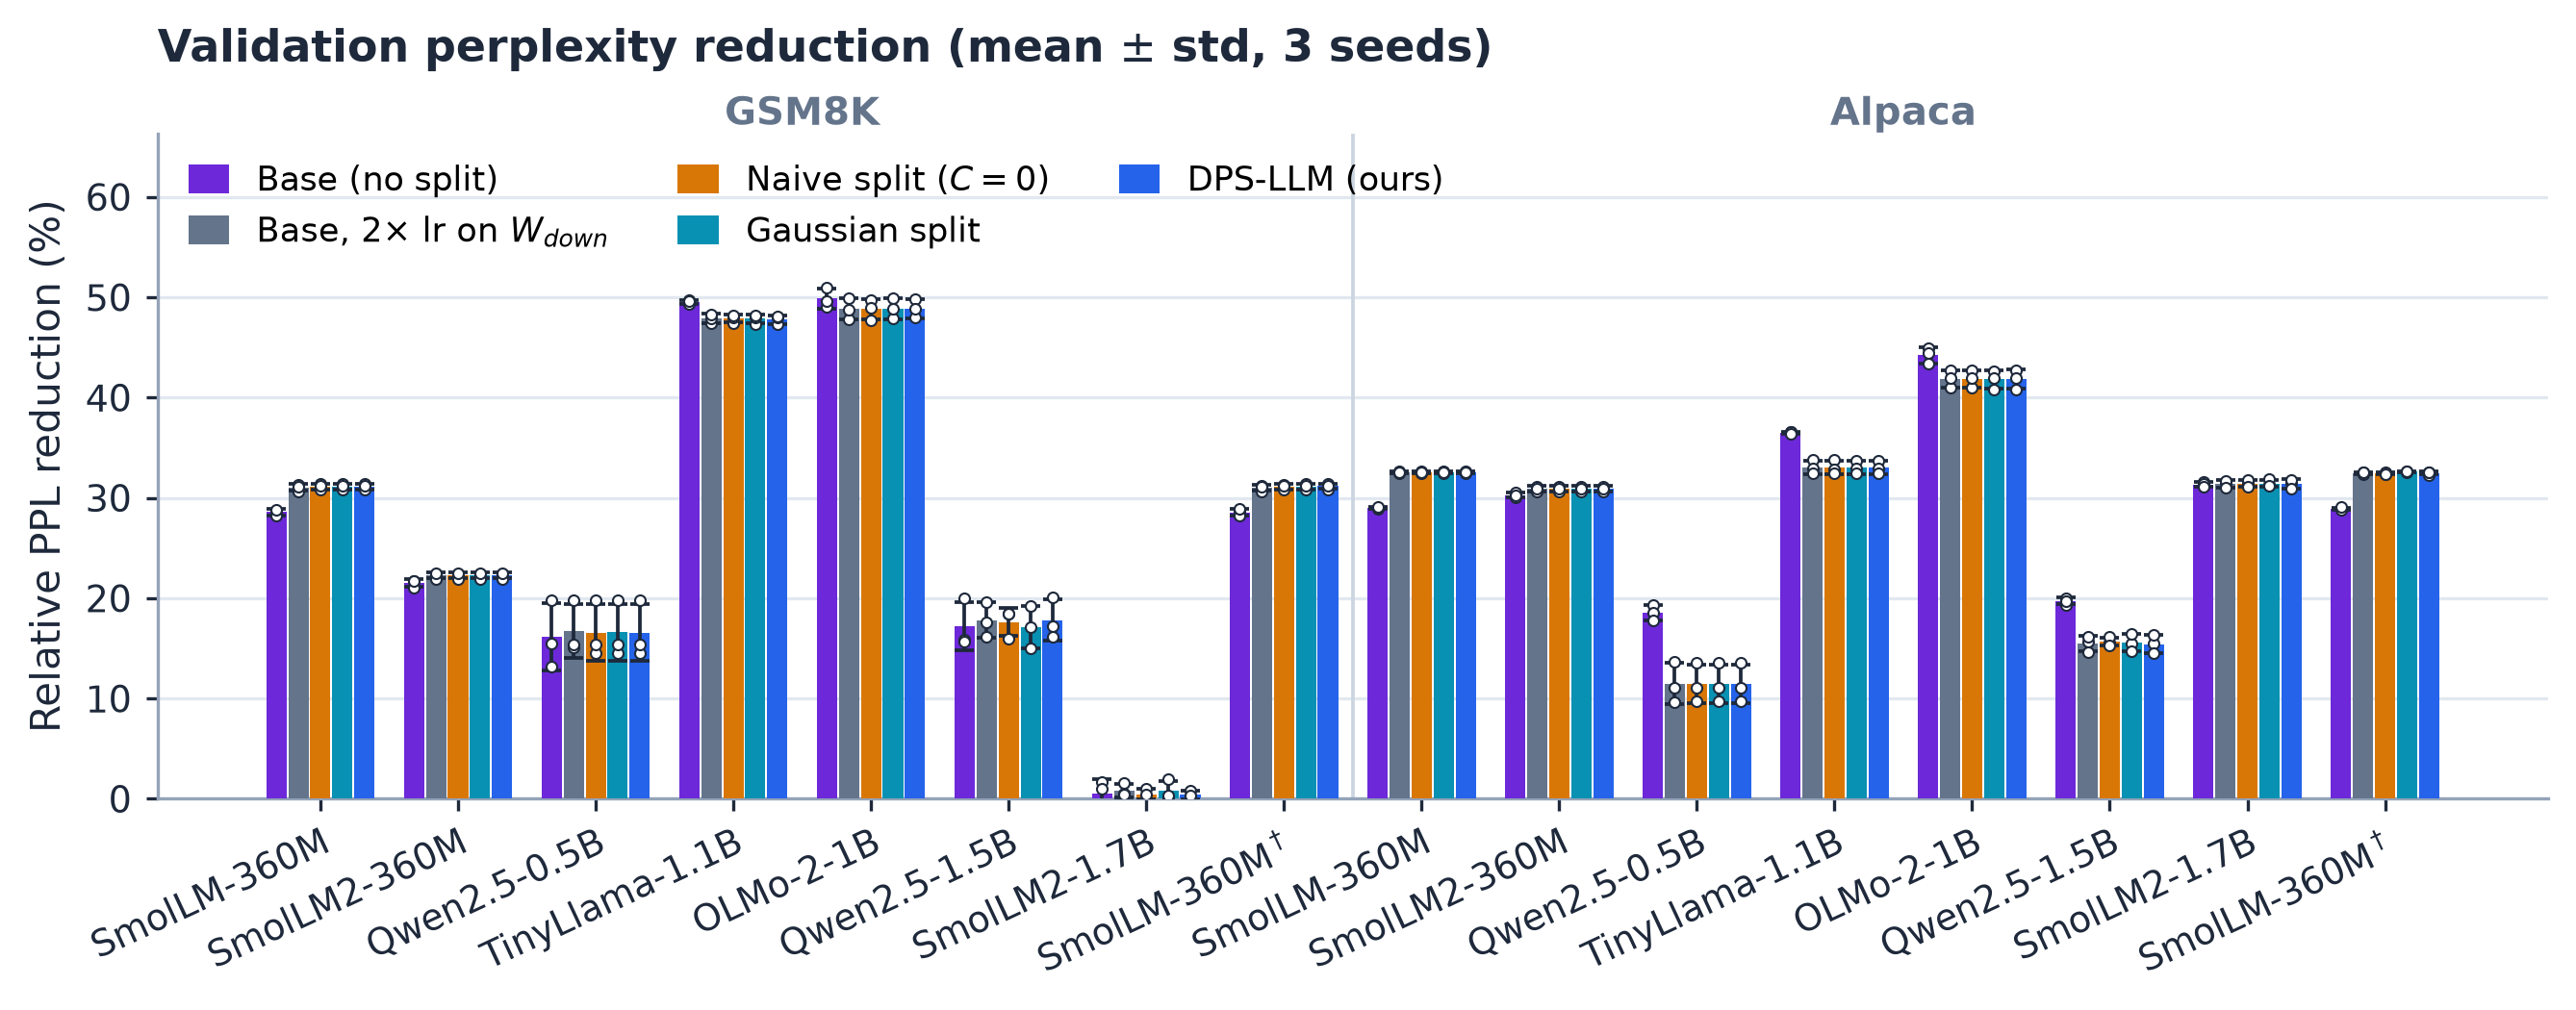
\includegraphics[width=\textwidth]{multi_model_benchmark_comparison.png}
    \caption{\textbf{Benchmark summary}: relative validation-perplexity reduction, mean $\pm$ std over three seeds, with individual seeds as dots. In every setting the three splits (orange, teal, blue) match the matched control (grey), whether they are above or below the unexpanded seed (purple). $^\dagger$: bfloat16 with stochastic rounding.}
    \label{fig:benchmark_results}
\end{figure*}

\subsection{Results}
\label{sec:results}

\paragraph{The split is function-preserving, and the anti-symmetric pairing cancels drift.}
In float32, validation perplexity immediately after the DPS split differs from the seed's by at most $1.3\times10^{-6}$ across all runs, the same as exact duplication ($1.8\times10^{-6}$, from re-associating floating-point sums), whereas Gaussian noise of the same RMS shifts it by up to $2.1\times10^{-4}$. The ablation (Table~\ref{tab:ablation}) shows the same ordering at every noise scale: at $C{=}10^{-1}$ the DPS drift is $1.3\times10^{-3}$ against $1.5\times10^{-2}$ for Gaussian noise, and the anti-symmetric pairing removes the drift that a symmetric $(+\delta,+\delta)$ pairing leaves ($0$ vs.\ $3.0\times10^{-5}$ at $C{=}10^{-4}$), as Proposition~\ref{prop:drift} predicts. Removing the $\tfrac{1}{2}$ factor raises the initial perplexity from 5.13 to 14.47. Under the bfloat16 protocol the split is rounded to nearest, which alone shifts perplexity by up to 0.02.

\paragraph{A split behaves like a learning-rate change.}
In 15 of 18 settings each of the three splits ends within $0.18$ points of the matched control (Table~\ref{tab:empirical_results}, Figure~\ref{fig:benchmark_results}); the exceptions are three noisy GSM8K settings, Qwen2.5-1.5B, SmolLM2-1.7B and Llama-3.2-1B, where the splits are within $0.68$ points of the control and the seed standard deviation is $0.4$--$2.4$. Only one of eighteen DPS-vs-control comparisons reaches $p<0.05$ (SmolLM-360M/GSM8K, $+0.11$ points). Relative to the unexpanded seed at the shared learning rate, splitting looks helpful where the seed is learning-rate-limited (SmolLM-360M: $+2.6$ on GSM8K, $+3.6$ on Alpaca) and harmful where a larger step on $W_{down}$ overshoots (Qwen2.5-0.5B/Alpaca: $-7.1$; Qwen2.5-1.5B/Alpaca: $-4.3$; TinyLlama: $-1.8$ and $-3.5$; OLMo-2-1B: $-1.0$ and $-2.4$; Llama-3.2-1B: $-5.6$ and $-6.0$). The control moves by the same amounts in every case ($+2.5$, $+3.5$, $-7.1$, $-4.2$, $-1.7$, $-3.4$, $-1.0$, $-2.3$, $-5.6$, $-6.1$), so these differences are the step-size effect of Proposition~\ref{prop:lr}, not capacity.

\paragraph{The perturbation does not break the symmetry.}
In float32 the relative distance between paired neurons after 100 steps equals its value at the split to three significant digits ($5.84\times10^{-5}$ for DPS-LLM and $4.13\times10^{-5}$ for Gaussian noise on SmolLM-360M; Figure~\ref{fig:divergence}a), and exactly zero for naive duplication. Across the ablation the distance scales linearly with $C$ and never grows, and the final perplexity is identical to four significant digits for DPS-LLM at every $C\le10^{-2}$ and for Gaussian noise up to $C{=}10^{-3}$ (Table~\ref{tab:ablation}). This is consistent with Proposition~\ref{prop:lr}: a perturbation of relative size $C$ changes the two copies' gradients by $O(C)$, so Adam, whose update depends on the gradient's direction rather than its scale, moves both copies by almost the same step and the initial gap is preserved rather than amplified. Under the bfloat16 protocol, stochastic rounding of each update pulls the copies apart by itself, so even naive duplication reaches a distance of $3.6\times10^{-3}$ on SmolLM-360M (Figure~\ref{fig:divergence}b) and $5$--$12\times10^{-3}$, 64--89\% of the DPS-LLM distance, on the five models of 1B parameters and more; this still yields no consistent gain. Of the fifty-four pairwise comparisons among the three splits only one reaches $p<0.05$ (Gaussian over naive on SmolLM-360M$^\dagger$/Alpaca, $+0.21$ points), fewer than the 2.7 expected by chance.

\paragraph{At matched learning rates the larger model does not win.}
Table~\ref{tab:lr} compares each model's best learning rate for the seed and for DPS-LLM. The differences range from $-3.11$ to $+2.61$ points; the seed is ahead on six of nine settings. The two largest differences come from the largest models. On Qwen2.5-1.5B, DPS-LLM peaks at a lower rate than the seed and diverges at $10^{-4}$ ($-15.6\%$ against $+3.6\%$ for the seed), and on Llama-3.2-1B it degrades much faster than the seed at high rates ($-50.2\%$ against $-15.8\%$ at $10^{-4}$), as expected if the split doubles the effective step on $W_{down}$; on SmolLM2-1.7B both peak at the largest rate swept, so the sweep does not bracket its optimum. Within this budget, the 54--75\% of added parameters do not translate into a consistently lower perplexity.

\paragraph{Accuracy.}
GSM8K exact match on 50 problems is a coarse measure (Table~\ref{tab:accuracy}), but it shows the same pattern. Fine-tuning on reference solutions lowers the accuracy of Qwen2.5-0.5B from 22\% to 9.3\% for the seed and 4.7--5.3\% for the splits and the control, of OLMo-2-1B from 54\% to 16.0\% and 6.7--8.7\%, and of Llama-3.2-1B from 12\% to 3.3\% and 2.7--6.0\%. In all three, the splits stay within 2.6 points (fewer than two problems) of the control, consistent with a larger effective step on $W_{down}$ rather than with the split. The two largest models instead improve: Qwen2.5-1.5B from 12\% to 14.0--17.3\% and SmolLM2-1.7B from 14\% to 32.0--34.0\%, the latter while its GSM8K perplexity falls by less than 1\%, which suggests it mainly learns the answer format; in both, all five conditions lie within 3.3 points, fewer than two of the 50 problems.

\paragraph{Pilot in pure bfloat16.}
With round-to-nearest bfloat16, the $C{=}10^{-4}$ perturbation is absorbed by rounding: the two copies of every neuron kept a cosine similarity of $1.0000$ for 200 steps, and DPS-LLM, Gaussian noise and duplication were statistically indistinguishable ($p\ge0.09$). An emulation of bfloat16 rounding on $\mathcal{N}(0,0.02^2)$ weights shows why: at $C{=}10^{-4}$ the copies differ in only 0.6\% of entries, against 42\% at $C{=}10^{-2}$. The same run also lost most small updates, since an update of $2\times10^{-5}$ is below half a bfloat16 ulp for most weights; SmolLM-360M's base model improved perplexity by 5.3\% in that run despite twice as many steps, against 28.6\% in float32 here.

\begin{figure}[t]
    \centering
    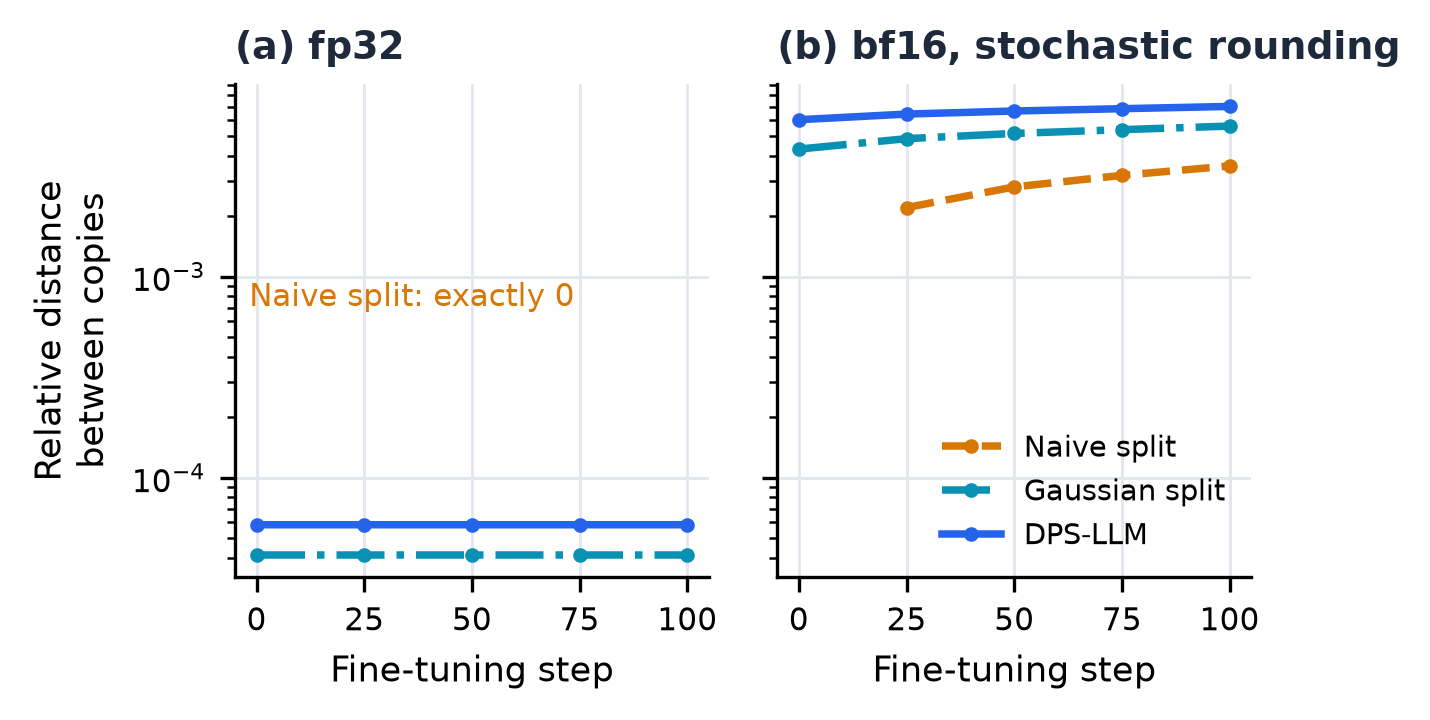
\includegraphics[width=\figwidth]{pair_divergence.png}
    \caption{\textbf{Distance between the two copies of each split neuron} during fine-tuning of SmolLM-360M, mean over seeds and datasets. In float32 (a) the gap created by the perturbation is preserved but never grows. Under bfloat16 with stochastic rounding (b) the rounding itself separates the copies, including for exact duplication.}
    \label{fig:divergence}
\end{figure}

\begin{table}[t]
\centering
\footnotesize
\setlength{\tabcolsep}{4pt}
\caption{\textbf{Best learning rate per model} (GSM8K, seed 42; sweep over $\{1,2,5,10\}\times10^{-5}$): relative perplexity reduction (\%) of the seed and of DPS-LLM, each at its own best rate.}
\label{tab:lr}
\begin{adjustbox}{max width=\columnwidth}\input{tables/lr.tex}\end{adjustbox}
\end{table}

\begin{table}[t]
\centering
\footnotesize
\setlength{\tabcolsep}{4pt}
\caption{\textbf{GSM8K exact-match accuracy (\%)} on 50 test problems before fine-tuning and after it (mean over seeds).}
\label{tab:accuracy}
\begin{adjustbox}{max width=\columnwidth}\input{tables/accuracy.tex}\end{adjustbox}
\end{table}

\begin{table}[t]
\centering
\footnotesize
\setlength{\tabcolsep}{3pt}
\caption{\textbf{Ablations} on SmolLM-360M/GSM8K, float32, seed 42, 50 steps. \emph{Init drift}: change of validation perplexity caused by the split (base: 5.13). \emph{Red.}: relative perplexity reduction after fine-tuning. \emph{Pair dist.}: relative distance between paired neurons after fine-tuning.}
\label{tab:ablation}
\begin{adjustbox}{max width=\columnwidth}\input{tables/ablation.tex}\end{adjustbox}
\end{table}

% -----------------------------------------------------------------------------
\section{Conclusion}
The function-preserving half of DPS-LLM works as designed: placing the factor $\tfrac{1}{2}$ on the down projection grows the SwiGLU blocks of a pre-trained LLM without changing its output, and the anti-symmetric, polarity-signed perturbation cancels first-order drift in practice, by two orders of magnitude relative to Gaussian noise. The symmetry-breaking half does not take effect during fine-tuning: the gap between paired neurons is preserved but never amplified, so the split model behaves like its seed, and under Adam that means like its seed with a doubled learning rate on $W_{down}$. A matched control reproduces every gain and loss we observe, and at each model's best learning rate the split model is not consistently better than the seed. We draw two lessons for work on model growth. Comparisons of a grown model with its seed at a shared learning rate conflate capacity with step size and need the matched control; and symmetry breaking should be verified by measuring whether the copies diverge, not assumed from the perturbation. Whether larger noise, longer training from scratch-scale budgets, or growth during pre-training changes this picture remains open; the same operator applies to MoE upcycling and LoRA rank growth, which we have not evaluated.

% -----------------------------------------------------------------------------
\section*{Limitations}
\textbf{Scale.} We evaluate eight models up to 1.7B parameters, fine-tuned for 50 optimiser updates on 256 examples; capacity effects may only appear with larger models, larger datasets or longer training, and in pre-training rather than fine-tuning.
\textbf{Statistics.} Three seeds per condition detect only differences of a few tenths of a point; the learning-rate sweep and the ablations use a single seed, and the sweep does not bracket the best rate of SmolLM2-1.7B.
\textbf{Precision.} The five models of 1B parameters and more use bfloat16 with stochastic rounding and a larger noise scale than the float32 models, so their noise condition is not identical; on SmolLM-360M the two protocols agree within $0.2$ points for every condition.
\textbf{Scope.} Only width splitting of the MLP was evaluated, with only the MLP parameters trainable; depth growth, attention-head splitting, the MoE and LoRA regimes, and full-parameter fine-tuning are untested. We measure perplexity and GSM8K exact match but not instruction-following quality for Alpaca-Cleaned.
\textbf{Data provenance.} The Alpaca-Cleaned validation examples come from its training split; they are unseen during our fine-tuning but may have been seen during the checkpoints' original training.

\section*{\ethicsheading}
This work modifies the architecture of publicly released language models and uses two public datasets (GSM8K, MIT licence; Alpaca-Cleaned, CC~BY-NC~4.0) and eight public checkpoints (Qwen2.5-0.5B-Instruct, Qwen2.5-1.5B-Instruct, SmolLM-360M-Instruct, SmolLM2-360M-Instruct, SmolLM2-1.7B-Instruct, TinyLlama-1.1B-Chat and OLMo-2-0425-1B-Instruct, all Apache~2.0; Llama-3.2-1B-Instruct, Llama~3.2 Community License, used under its terms for research). Growing a model does not change the biases or safety properties of its seed, and a grown model inherits any limitations of the original checkpoint; practitioners should re-run their safety evaluations after expansion. All experiments ran on a free cloud GPU tier with a small compute footprint (about 23 hours on a two-T4 instance for the benchmark, sweeps and ablations, and 4 for the pilot). No human subjects or personal data were involved.

\ifdefined\FINAL\def\showacknowledgements{}\fi
\ifdefined\ARXIV\def\showacknowledgements{}\fi
\ifdefined\showacknowledgements
\section*{Acknowledgements}
The author thanks Dr.~M.~Ali Tahir (SEECS, National University of Sciences and Technology) for supervising the thesis on which this work builds.
\fi
:
\providecommand{\figwidth}{\columnwidth}          % width of single-column figures
\providecommand{\appref}[1]{Appendix~\ref{#1}}   % IJCAI: appendix is supplementary
\providecommand{\ethicsheading}{Ethics Statement} % ICML: Impact Statement

\begin{abstract}
Growing a pre-trained large language model (LLM) in place, instead of training a larger one from scratch, needs an expansion that preserves the model's function and a way to make the added parameters useful.
We study \textbf{Discriminative Parameter Splitting for LLMs (DPS-LLM)}, which doubles the intermediate width of every SwiGLU feed-forward block by duplicating the gate and up projections and the $\tfrac{1}{2}$-scaled down projection, and breaks the symmetry of the copies with a polarity-preserving, anti-symmetric perturbation adapted from LSTM acoustic models.
We prove that the split is exactly function-preserving and that the anti-symmetric pairing cancels first-order output drift, and confirm both on eight open-weight models from 360M to 1.7B parameters: in float32, the DPS split changes validation perplexity by at most $1.3\times10^{-6}$, two orders of magnitude less than Gaussian noise of the same size.
Its effect on fine-tuning is not what growth methods assume. We prove that under Adam an exact split trains like its seed with a doubled learning rate on the down projection, and a matched control, the unexpanded model with that learning rate, reproduces the split's perplexity reduction on every model and dataset, within $0.18$ points in 15 of 18 settings and within seed noise in the other three.
The perturbation does not break the symmetry: in float32 the distance between paired neurons stays constant during fine-tuning, and DPS-LLM, Gaussian noise and exact duplication are statistically indistinguishable. At each model's best learning rate, the split model, 54--75\% larger, is ahead of its seed on only three of nine settings.
We release code, notebooks and all per-seed results, and argue that evaluations of model growth need matched learning-rate controls.
\end{abstract}

% -----------------------------------------------------------------------------
\section{Introduction}
Transformer LLMs \citep{vaswani2017attention,touvron2023llama,qwen2024technical} are almost always trained under a \emph{static} paradigm: every dimension of the network is fixed \textit{a priori}, the weights are drawn from a random initialization \citep{glorot2010understanding,he2015delving}, and the model is trained end-to-end.
Scaling laws \citep{kaplan2020scaling,hoffmann2022chinchilla} make the cost of this paradigm explicit: a larger model must be trained from scratch, spending much of its early budget on features a smaller model already possesses.
The same rigidity appears at fine-tuning time. When a compact model saturates its parametric capacity on a domain-specific task, practitioners must either accept the plateau or restart with a larger architecture.

Progressive growth offers an alternative: begin with a compact \emph{seed} model and enlarge it during training \citep{chen2015net2net,gong2019stacking,chen2022bert2bert,wang2023ligo}.
Two requirements make growth practical for modern LLMs.
First, the expansion must be \emph{function-preserving}, so that the grown model neither loses the seed's knowledge nor suffers a loss spike.
Second, the duplicated parameters must be \emph{distinguishable}; otherwise identical copies receive identical gradients and the added capacity is never used \citep{chen2015net2net}.
Existing work on Transformers has addressed these requirements for pre-LayerNorm blocks with ReLU or GELU feed-forward layers \citep{chen2022bert2bert,wang2024lemon}, but gated SwiGLU blocks \citep{shazeer2020glu}, which are now standard in LLaMA, Mistral, Gemma, Qwen and SmolLM, multiply two projections element-wise, so naive duplication doubles the block's output.

We adapt \emph{Discriminative Parameter Splitting} \citep{irfan2021discriminative}, originally developed for growing LSTM acoustic models, to SwiGLU Transformers, and ask whether it delivers on both requirements when a pre-trained LLM is fine-tuned. Our contributions are:
\begin{itemize}
    \item \textbf{An exact function-preserving SwiGLU split with drift-cancelling noise.} Duplicating the rows of $W_{gate}$ and $W_{up}$ and the columns of $\tfrac{1}{2}W_{down}$ doubles $d_{ffn}$ with provably identical output (Theorem~\ref{thm:invariance}), and a polarity-signed, anti-symmetric perturbation cancels first-order drift (Proposition~\ref{prop:drift}). Both hold on real checkpoints.
    \item \textbf{A split is a learning-rate change.} Under Adam, an exact split trains like its seed with a doubled learning rate on $W_{down}$ (Proposition~\ref{prop:lr}). We introduce the matched control this implies and show that it reproduces the split's gains.
    \item \textbf{A controlled benchmark.} On eight open-weight models from four families (360M--1.7B), two datasets, five conditions, three seeds, per-model learning-rate sweeps and ablations, we find no gain from added capacity and no symmetry breaking during fine-tuning.
    \item \textbf{A precision pitfall.} In bfloat16 the default perturbation is rounded away entirely; we give a stochastic-rounding protocol under which it survives.
\end{itemize}
We also describe, and release code for, two further regimes of the same operator---dense-to-Mixture-of-Experts (MoE) upcycling and LoRA rank doubling---which we leave for empirical evaluation in future work (\appref{app:regimes}).

\begin{figure}[t]
    \centering
    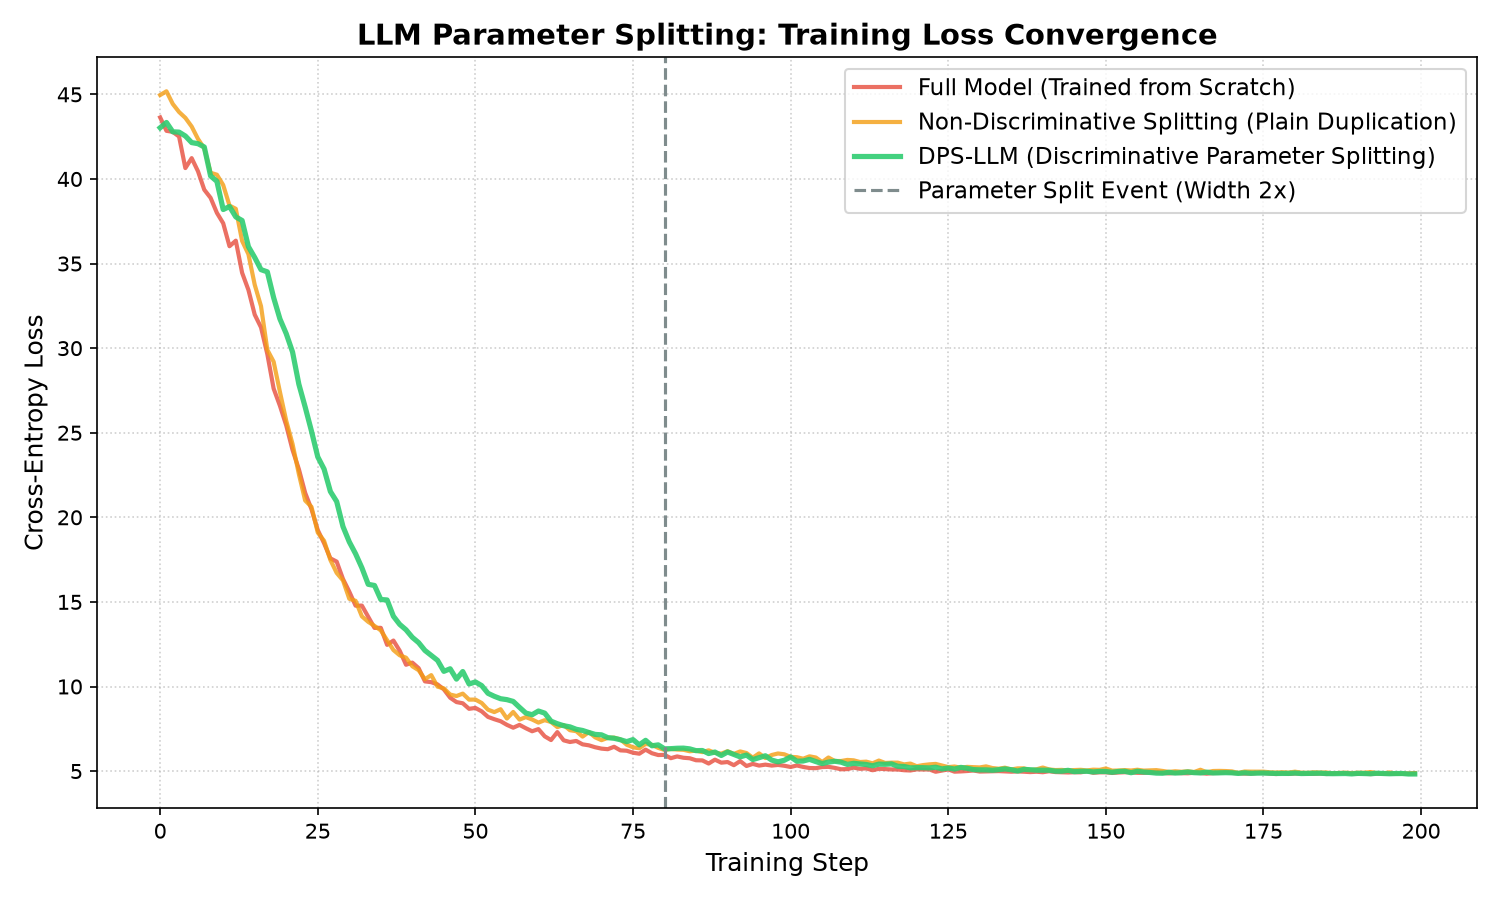
\includegraphics[width=\figwidth]{dps_llm_training_curve.png}
    \caption{\textbf{Controlled split on a synthetic language-modelling task.} A two-layer SwiGLU Transformer with $d_{ffn}=64$ is trained for 80 steps and then split to $d_{ffn}=128$ (dashed line). Both split variants continue without a loss spike, whereas the $d_{ffn}=128$ model trained from scratch spends its first 80 steps re-learning what the seed already knows. DPS-LLM and plain duplication converge to the same loss as the full model by step 200.}
    \label{fig:training_curve}
\end{figure}

% -----------------------------------------------------------------------------
\section{Related Work}
\paragraph{Function-preserving growth.}
Net2Net \citep{chen2015net2net} introduced \emph{Net2WiderNet} and \emph{Net2DeeperNet}, which widen or deepen a network without changing its function, and noted that a small amount of noise is needed to break the symmetry of copied units. Network morphism \citep{wei2016morphism} generalised the idea to arbitrary non-linear morphisms.
For Transformers, progressive stacking \citep{gong2019stacking} and staged training \citep{shen2022staged} grow depth and width of BERT-style encoders; bert2BERT \citep{chen2022bert2bert} extends Net2Net to attention blocks with function-preserving and advanced knowledge initialisation; LiGO \citep{wang2023ligo} learns a linear growth operator from the small model; MSG \citep{yao2024msg} and LEMON \citep{wang2024lemon} obtain lossless expansion for pre-LayerNorm blocks by masking or by an explicit average-and-cancel construction.
Depth up-scaling \citep{kim2024solar} and HyperCloning \citep{samragh2024hypercloning} apply the same principle to decoder-only LLMs, the latter by tiling weights of a small model into a wider one.
DPS-LLM belongs to this family but targets the gated SwiGLU block specifically, where the $\tfrac{1}{2}$ factor must be placed on the down projection to preserve function.

\paragraph{Neuron splitting.}
Splitting steepest descent \citep{liu2019splitting}, Firefly descent \citep{wu2020firefly} and GradMax \citep{evci2022gradmax} choose \emph{which} neurons to split and \emph{how} to perturb the copies using second-order or gradient information. These methods are principled but require extra computation per split; DPS-LLM instead splits every neuron and uses a closed-form, gradient-free perturbation whose only statistic is the standard deviation of the weight matrix.

\paragraph{Mixture-of-Experts upcycling.}
Sparse upcycling \citep{komatsuzaki2022sparse} initialises MoE experts \citep{shazeer2017outrageously,lepikhin2021gshard,fedus2022switch} by cloning a dense MLP, and \citet{he2024upcycling} study this recipe at scale; Mixtral \citep{jiang2024mixtral} is a widely used dense-to-sparse architecture. Cloned experts are initially identical, so the same symmetry problem arises; our anti-symmetric noise is directly applicable (\appref{app:regimes}).

\paragraph{Adapter rank growth.}
LoRA \citep{hu2021lora} fixes the adapter rank in advance; AdaLoRA \citep{zhang2023adalora} and DyLoRA \citep{valipour2023dylora} adapt the rank during training. Rank doubling by parameter splitting (\appref{app:regimes}) is a complementary, function-preserving way to increase adapter capacity.

\paragraph{Discriminative splitting in speech.}
\citet{irfan2021discriminative} grew LSTM-RNN acoustic models by duplicating rows and columns of weight matrices and injecting a polarity-preserving perturbation, reporting faster convergence, less over-training and a 1.2\% absolute word-error-rate reduction over Xavier initialisation on a Kaldi/VoxForge recipe. This paper transfers that recipe to Transformers and adds the invariance scaling and the anti-symmetric pairing.

% -----------------------------------------------------------------------------
\section{Method}
\subsection{Function-preserving SwiGLU width splitting}
\label{sec:split}
Modern decoder blocks \citep{shazeer2020glu,touvron2023llama,qwen2024technical} use a gated feed-forward network
\begin{equation}
    \mathrm{FFN}(x) = W_{down}\,\big(\mathrm{SiLU}(W_{gate}x) \odot W_{up}x\big),
    \label{eq:swiglu}
\end{equation}
with $W_{gate},W_{up}\in\mathbb{R}^{d_{ffn}\times d_{model}}$, $W_{down}\in\mathbb{R}^{d_{model}\times d_{ffn}}$, and $\mathrm{SiLU}(z)=z\,\sigma(z)$ \citep{hendrycks2016gelu,elfwing2018silu,ramachandran2017swish}. Let $h(x)=\mathrm{SiLU}(W_{gate}x)\odot W_{up}x\in\mathbb{R}^{d_{ffn}}$.

To grow $d_{ffn}\to 2d_{ffn}$ we apply \emph{rows extension} to the two incoming projections and \emph{columns extension} with a $\tfrac{1}{2}$ factor to the outgoing projection:
\begin{align}
    W_{gate}^{\prime} &= \begin{bmatrix} W_{gate}+\Delta_{gate}^{(1)} \\ W_{gate}+\Delta_{gate}^{(2)} \end{bmatrix}, \label{eq:rows}\\
    W_{up}^{\prime} &= \begin{bmatrix} W_{up}+\Delta_{up}^{(1)} \\ W_{up}+\Delta_{up}^{(2)} \end{bmatrix}, \label{eq:rows_up}\\
    W_{down}^{\prime} &= \tfrac{1}{2}\begin{bmatrix} W_{down} & W_{down} \end{bmatrix} \nonumber\\
    &\quad + \begin{bmatrix} \Delta_{down}^{(1)} & \Delta_{down}^{(2)} \end{bmatrix}. \label{eq:cols}
\end{align}

\begin{theorem}[Functional invariance]
\label{thm:invariance}
With $\Delta=0$, $\mathrm{FFN}'(x)=\mathrm{FFN}(x)$ for every input $x$.
\end{theorem}
\begin{proof}
The stacked gate and up projections produce $[h(x);\,h(x)]$, so
$\mathrm{FFN}'(x)=\tfrac{1}{2}W_{down}h(x)+\tfrac{1}{2}W_{down}h(x)=W_{down}h(x)$.
\end{proof}
Because every block is invariant and the residual stream, attention and normalisation layers are untouched, the whole model is invariant; the loss on any batch is unchanged in exact arithmetic. Without the $\tfrac{1}{2}$ factor the block's output would double, which is the loss spike observed when SwiGLU networks are naively widened.

\subsection{Calculated Anti-Symmetric Noise}
\label{sec:noise}
If $\Delta=0$, the two copies of every neuron are identical and receive identical gradients for the rest of training, so the expanded model has no more effective capacity than the seed \citep{chen2015net2net}.
Isotropic Gaussian noise breaks the tie but is sign-agnostic: it flips the polarity of small weights, which \citet{irfan2021discriminative} found harmful for pre-trained LSTMs.
We instead use a perturbation whose sign is dictated by the weight it perturbs. For a weight matrix $W$ with element-wise standard deviation $\sigma_W$, draw $u\sim\mathcal{U}(0,1)$ and $n\sim\mathcal{N}(0,1)$ independently per element and set
\begin{align}
    f(W) &= \big|(u-\tfrac{1}{2})\cdot C\,\sigma_W\cdot n\big|, \label{eq:f}\\
    \delta(W) &= \mathrm{sign}(W)\odot f(W), \label{eq:delta}\\
    \Delta^{(1)} &= +\delta(W), \qquad \Delta^{(2)} = -\delta(W). \label{eq:pair}
\end{align}
The modulation constant $C=10^{-4}$ is inherited from the original speech recipe; \eqref{eq:f}--\eqref{eq:delta} are its Equations 5.7--5.8 with the noise scaled by $\sigma_W$ so that the same $C$ transfers across layers of different magnitude. Equation~\eqref{eq:pair} is new: the two copies receive \emph{opposite} perturbations. For $W_{down}$ the noise is computed on the already-halved matrix.

\begin{proposition}[Sign preservation]
\label{prop:sign}
Copy 1 satisfies $|w+\delta(w)|=|w|+f(w)>|w|$ for every weight, so no sign is flipped. Copy 2 satisfies $|w-\delta(w)|=\big||w|-f(w)\big|$ and flips sign only if $|w|<f(w)$.
\end{proposition}
Since $f(w)\leq\tfrac{1}{2}C\sigma_W|n|$, a flip requires $|w|<\tfrac{1}{2}\cdot10^{-4}\sigma_W|n|$; for approximately Gaussian weights this is a fraction on the order of $10^{-4}$ of the matrix or less, and these weights carry negligible signal. In our runs the measured sign-flip fraction is $8$--$9\times10^{-6}$ (Section~\ref{sec:results}).

\begin{proposition}[First-order drift cancellation]
\label{prop:drift}
With the pairing in \eqref{eq:pair}, $\mathrm{FFN}'(x)=\mathrm{FFN}(x)+O(\|\delta\|^2)$.
\end{proposition}
\begin{proof}
Write $h_{1}(x)$ and $h_{2}(x)$ for the hidden activations of the two copies. A first-order expansion in $\delta$ gives $h_{1}=h+J\delta x+O(\delta^2)$ and $h_{2}=h-J\delta x+O(\delta^2)$ for the same Jacobian $J$, so $\tfrac{1}{2}W_{down}(h_{1}+h_{2})=W_{down}h+O(\delta^2)$. The down-projection perturbation contributes $\delta_{down}h_{1}-\delta_{down}h_{2}=\delta_{down}(h_{1}-h_{2})=O(\delta^2)$.
\end{proof}
The perturbation therefore does two things at once: it leaves the output unchanged to first order, and it makes $\nabla_{W^{(1)}}\mathcal{L}\neq\nabla_{W^{(2)}}\mathcal{L}$ from the very first update, because the two copies now see different pre-activations. Both statements assume that the perturbation is representable in the weight format. bfloat16 keeps 8 significant bits, so a perturbation of relative size $10^{-4}$ is rounded away for all but the smallest weights; Section~\ref{sec:results} shows that this is what happens in practice.

\subsection{An exact split changes the effective learning rate}
\label{sec:lr_equiv}
Function preservation holds at the moment of the split, but not along the optimisation trajectory. With Adam-type optimisers \citep{kingma2015adam,loshchilov2019adamw}, the split also changes the effective step size of the block.
\begin{proposition}[Split as learning-rate doubling]
\label{prop:lr}
Let the split be exact ($\Delta=0$) and let both models be trained with Adam at learning rate $\eta$. Then, up to Adam's $\epsilon$, the copies stay identical and the split model follows the trajectory of the unsplit model trained with learning rate $\eta$ on $W_{gate},W_{up}$ and $2\eta$ on $W_{down}$.
\end{proposition}
\begin{proof}[Proof sketch]
While the copies are identical, each copy of a row of $W_{gate}$ or $W_{up}$ receives exactly half the gradient of the original row, because it feeds a down-projection column scaled by $\tfrac{1}{2}$; Adam's update is invariant to a constant rescaling of the gradient, so both copies take the step the original would take, and stay identical. Each copy of a column of $W_{down}$ receives the full gradient of the original column, because it sees the same activation; both copies take the original's step, and the effective matrix $W^{(1)}_{down}+W^{(2)}_{down}$ moves twice as far.
\end{proof}
The equivalence is exact in exact arithmetic without gradient clipping and with decoupled weight decay ignored; global-norm clipping, which rescales all gradients jointly, and finite precision make it approximate. On a toy SwiGLU block trained with AdamW in float32 for 100 steps, the losses of the exact split and of the unsplit block with a $2\times$ learning rate on $W_{down}$ differ by at most $7\times10^{-6}$, against $2.4\times10^{-2}$ from the unsplit block at the original learning rate. Comparisons between a split model and its seed at one shared learning rate therefore conflate added capacity with a larger step on $W_{down}$; Section~\ref{sec:results} confirms the equivalence on real checkpoints.

\subsection{Applying the operator to a pre-trained LLM}
The split is applied in place to every decoder layer of a Hugging Face checkpoint \citep{wolf2020transformers}: the three linear layers are replaced by their expanded versions and \texttt{intermediate\_size} is doubled in the configuration. No other tensors change. For Qwen2.5-0.5B this grows $d_{ffn}$ from 4864 to 9728 in all 24 layers (+313.8M parameters); for SmolLM-360M from 2560 to 5120 in all 32 layers (+236.0M).

% -----------------------------------------------------------------------------
\begin{table*}[t]
\centering
\small
\setlength{\tabcolsep}{3pt}
\caption{\textbf{Relative validation-perplexity reduction (\%) after fine-tuning}, mean{\scriptsize$\pm$std} over three seeds (higher is better; bold: best mean per row). \emph{Base, 2$\times$ lr $W_{down}$} is the unexpanded model trained with a doubled learning rate on the down projection, the matched control of Proposition~\ref{prop:lr}. \emph{DPS $-$ ctrl}: mean paired difference between DPS-LLM and the control, with the paired $t$-test $p$-value. Models without a mark are fine-tuned in float32 with $C{=}10^{-4}$; $^\dagger$: bfloat16 with stochastic rounding and $C{=}10^{-2}$.}
\label{tab:empirical_results}
\vspace{2pt}
\begin{adjustbox}{max width=\textwidth}\begin{tabular}{@{}llcccccc@{}}
\toprule
\textbf{Model} & \textbf{Data} & \textbf{Base} & \textbf{Base, 2$\times$ lr $W_{down}$} & \textbf{Naive split} & \textbf{Gaussian split} & \textbf{DPS-LLM} & \textbf{DPS $-$ ctrl ($p$)} \\
\midrule
SmolLM-360M & GSM8K & 28.58{\scriptsize$\pm$0.30} & 31.04{\scriptsize$\pm$0.32} & \textbf{31.15{\scriptsize$\pm$0.30}} & \textbf{31.15{\scriptsize$\pm$0.30}} & \textbf{31.15{\scriptsize$\pm$0.30}} & +0.11 (0.04) \\
SmolLM2-360M & GSM8K & 21.51{\scriptsize$\pm$0.39} & 22.28{\scriptsize$\pm$0.32} & \textbf{22.29{\scriptsize$\pm$0.32}} & \textbf{22.29{\scriptsize$\pm$0.32}} & \textbf{22.29{\scriptsize$\pm$0.32}} & +0.01 (0.12) \\
Qwen2.5-0.5B & GSM8K & 16.12{\scriptsize$\pm$3.35} & \textbf{16.75{\scriptsize$\pm$2.66}} & 16.58{\scriptsize$\pm$2.86} & 16.60{\scriptsize$\pm$2.83} & 16.58{\scriptsize$\pm$2.86} & $-$0.17 (0.50) \\
TinyLlama-1.1B$^\dagger$ & GSM8K & \textbf{49.55{\scriptsize$\pm$0.21}} & 47.88{\scriptsize$\pm$0.45} & 47.86{\scriptsize$\pm$0.38} & 47.85{\scriptsize$\pm$0.46} & 47.79{\scriptsize$\pm$0.43} & $-$0.09 (0.41) \\
Llama-3.2-1B$^\dagger$ & GSM8K & \textbf{31.95{\scriptsize$\pm$0.96}} & 26.34{\scriptsize$\pm$2.08} & 26.80{\scriptsize$\pm$1.55} & 26.59{\scriptsize$\pm$2.02} & 26.37{\scriptsize$\pm$2.02} & +0.03 (0.74) \\
OLMo-2-1B$^\dagger$ & GSM8K & \textbf{49.88{\scriptsize$\pm$1.00}} & 48.83{\scriptsize$\pm$1.04} & 48.82{\scriptsize$\pm$1.00} & 48.85{\scriptsize$\pm$1.01} & 48.89{\scriptsize$\pm$0.95} & +0.06 (0.39) \\
Qwen2.5-1.5B$^\dagger$ & GSM8K & 17.20{\scriptsize$\pm$2.41} & 17.79{\scriptsize$\pm$1.77} & 17.62{\scriptsize$\pm$1.40} & 17.12{\scriptsize$\pm$2.10} & \textbf{17.83{\scriptsize$\pm$2.03}} & +0.03 (0.90) \\
SmolLM2-1.7B$^\dagger$ & GSM8K & 0.55{\scriptsize$\pm$1.41} & \textbf{0.82{\scriptsize$\pm$0.67}} & 0.46{\scriptsize$\pm$0.55} & 0.79{\scriptsize$\pm$0.99} & 0.40{\scriptsize$\pm$0.42} & $-$0.42 (0.19) \\
SmolLM-360M$^\dagger$ & GSM8K & 28.57{\scriptsize$\pm$0.33} & 31.03{\scriptsize$\pm$0.31} & 31.12{\scriptsize$\pm$0.27} & 31.14{\scriptsize$\pm$0.29} & \textbf{31.16{\scriptsize$\pm$0.29}} & +0.13 (0.07) \\
\midrule
SmolLM-360M & Alpaca & 29.02{\scriptsize$\pm$0.08} & 32.55{\scriptsize$\pm$0.10} & \textbf{32.58{\scriptsize$\pm$0.09}} & \textbf{32.58{\scriptsize$\pm$0.09}} & \textbf{32.58{\scriptsize$\pm$0.09}} & +0.03 (0.14) \\
SmolLM2-360M & Alpaca & 30.27{\scriptsize$\pm$0.23} & \textbf{30.91{\scriptsize$\pm$0.28}} & \textbf{30.91{\scriptsize$\pm$0.29}} & \textbf{30.91{\scriptsize$\pm$0.29}} & \textbf{30.91{\scriptsize$\pm$0.29}} & +0.00 (0.62) \\
Qwen2.5-0.5B & Alpaca & \textbf{18.56{\scriptsize$\pm$0.73}} & 11.47{\scriptsize$\pm$2.07} & 11.47{\scriptsize$\pm$1.95} & 11.47{\scriptsize$\pm$1.95} & 11.47{\scriptsize$\pm$1.95} & +0.00 (0.96) \\
TinyLlama-1.1B$^\dagger$ & Alpaca & \textbf{36.51{\scriptsize$\pm$0.08}} & 33.07{\scriptsize$\pm$0.67} & 33.05{\scriptsize$\pm$0.65} & 33.04{\scriptsize$\pm$0.63} & 33.04{\scriptsize$\pm$0.63} & $-$0.03 (0.25) \\
Llama-3.2-1B$^\dagger$ & Alpaca & \textbf{38.36{\scriptsize$\pm$0.09}} & 32.24{\scriptsize$\pm$0.46} & 32.26{\scriptsize$\pm$0.45} & 32.30{\scriptsize$\pm$0.51} & 32.36{\scriptsize$\pm$0.35} & +0.13 (0.30) \\
OLMo-2-1B$^\dagger$ & Alpaca & \textbf{44.22{\scriptsize$\pm$0.79}} & 41.89{\scriptsize$\pm$0.85} & 41.88{\scriptsize$\pm$0.87} & 41.81{\scriptsize$\pm$0.92} & 41.82{\scriptsize$\pm$0.97} & $-$0.07 (0.42) \\
Qwen2.5-1.5B$^\dagger$ & Alpaca & \textbf{19.71{\scriptsize$\pm$0.34}} & 15.50{\scriptsize$\pm$0.78} & 15.68{\scriptsize$\pm$0.40} & 15.54{\scriptsize$\pm$0.87} & 15.43{\scriptsize$\pm$0.88} & $-$0.07 (0.55) \\
SmolLM2-1.7B$^\dagger$ & Alpaca & 31.34{\scriptsize$\pm$0.25} & 31.42{\scriptsize$\pm$0.37} & \textbf{31.45{\scriptsize$\pm$0.37}} & \textbf{31.45{\scriptsize$\pm$0.35}} & 31.41{\scriptsize$\pm$0.45} & $-$0.01 (0.78) \\
SmolLM-360M$^\dagger$ & Alpaca & 28.92{\scriptsize$\pm$0.14} & 32.49{\scriptsize$\pm$0.10} & 32.42{\scriptsize$\pm$0.10} & \textbf{32.63{\scriptsize$\pm$0.06}} & 32.47{\scriptsize$\pm$0.15} & $-$0.02 (0.61) \\
\bottomrule
\end{tabular}
\end{adjustbox}
\end{table*}

\section{Experiments}
\subsection{Setup}
\label{sec:setup}
\paragraph{Models and precision.}
We use eight instruction-tuned open-weight checkpoints with SwiGLU blocks of the form \eqref{eq:swiglu}: SmolLM-360M, SmolLM2-360M and SmolLM2-1.7B \citep{allal2024smollm,allal2025smollm2}, Qwen2.5-0.5B and Qwen2.5-1.5B \citep{qwen2024technical}, TinyLlama-1.1B \citep{zhang2024tinyllama}, Llama-3.2-1B \citep{grattafiori2024llama3}, and OLMo-2-1B \citep{olmo2024olmo2}. The three models below 1B parameters are fine-tuned entirely in float32, where the $C{=}10^{-4}$ perturbation is representable. Models of 1B parameters and more are fine-tuned in bfloat16 to stay within the memory of two 16\,GB GPUs after splitting, with bfloat16 weights, an AdamW update computed in float32 and written back with stochastic rounding \citep{gupta2015deep,zamirai2020revisiting} (so updates smaller than half a unit in the last place are applied in expectation), and $C{=}10^{-2}$, because the split itself is rounded to nearest and a $C{=}10^{-4}$ perturbation would survive in only 0.6\% of entries (Section~\ref{sec:results}). To compare the two protocols on one checkpoint, SmolLM-360M is also run under the bfloat16 protocol (marked $^\dagger$).

\paragraph{Data.}
GSM8K \citep{cobbe2021gsm8k} and Alpaca-Cleaned \citep{taori2023alpaca,yahma2023alpacacleaned}, rendered with fixed templates (\appref{app:prompts}). For GSM8K we fine-tune on 256 examples drawn from the training split and measure perplexity on the first 100 test problems. For Alpaca-Cleaned, which has no test split, a fixed permutation of the training split provides 256 fine-tuning and 100 disjoint validation examples. GSM8K accuracy is exact match of the final number, generated greedily (at most 256 new tokens) for the first 50 test problems, before fine-tuning once per model and after fine-tuning for every run.

\paragraph{Conditions.}
(1) \emph{Base}: the unmodified checkpoint. (2) \emph{Base, 2$\times$ lr $W_{down}$}: the unmodified checkpoint with a doubled learning rate on every down projection, the matched control of Proposition~\ref{prop:lr}. (3) \emph{Naive split}: Eqs.~\eqref{eq:rows}--\eqref{eq:cols} with $\Delta{=}0$. (4) \emph{Gaussian split}: i.i.d.\ Gaussian noise drawn independently for each copy, as in Net2Net \citep{chen2015net2net}, with standard deviation $C\sigma_W/\sqrt{12}$ so that its RMS matches the calculated noise. (5) \emph{DPS-LLM}: Calculated Anti-Symmetric Noise.

\paragraph{Fine-tuning and evaluation.}
All conditions share one recipe (Table~\ref{tab:hparams}); only the SwiGLU parameters are trained, so the comparison isolates the expanded block. Validation perplexity \citep{jelinek1977perplexity} is $\exp$ of the mean per-sequence cross-entropy, measured before the first and after the last update. Every condition is run with seeds 42, 43 and 44, which set the noise draw and the order of the training examples; we report mean$\pm$std and paired $t$-tests across seeds. Every 25 steps we record the mean relative distance $\|a-b\|/\tfrac{1}{2}(\|a\|+\|b\|)$ between the two copies of every split neuron (rows of $W_{gate}$, $W_{up}$; columns of $W_{down}$). A \emph{learning-rate sweep} runs Base and DPS-LLM at $\{1,2,5,10\}\times10^{-5}$ on GSM8K (seed 42), and \emph{ablations} on SmolLM-360M/GSM8K (float32, seed 42, 50 steps) vary the noise scale, the pairing and the $\tfrac{1}{2}$ factor.

\paragraph{Pilot in pure bfloat16.}
An earlier run used pure bfloat16 with round-to-nearest updates, no matched control, Qwen2.5-0.5B and SmolLM-360M, and a 200-step budget. Its results are summarised at the end of Section~\ref{sec:results}; all per-seed data are released.

\begin{table}[t]
\centering
\footnotesize
\setlength{\tabcolsep}{4pt}
\caption{Fine-tuning recipe shared by all benchmark runs.}
\label{tab:hparams}
\begin{tabular}{@{}lp{0.62\columnwidth}@{}}
\toprule
\textbf{Setting} & \textbf{Value} \\
\midrule
Hardware & Kaggle, 2$\times$ NVIDIA T4 (16\,GB); runs sequential; layers of the ${\geq}$1B models spread over both GPUs \\
Precision & float32; or bfloat16 weights with stochastic-rounding AdamW ($^\dagger$) \\
Optimiser & AdamW \citep{loshchilov2019adamw}, $\beta{=}(0.9,0.999)$, weight decay $0.01$ \\
Learning rate & $2\times10^{-5}$, constant, no warm-up ($4\times10^{-5}$ on $W_{down}$ for the control) \\
Budget & 100 sequences (batch 1, accumulation 2 $\Rightarrow$ 50 updates) \\
Grad.\ clipping & global norm 1.0 \\
Max seq.\ length & 256 tokens \\
Trainable & SwiGLU MLP of every layer; rest frozen \\
Memory & gradient checkpointing \citep{chen2016checkpointing} \\
Noise constant & $C{=}10^{-4}$ (float32), $C{=}10^{-2}$ ($^\dagger$); $C{=}0$ (naive) \\
Data & 256 train / 100 validation sequences; 50 GSM8K test problems for accuracy \\
Seeds & 42, 43, 44 (noise draw, example order); data seed 0 \\
Software & PyTorch \citep{paszke2019pytorch}, Transformers \citep{wolf2020transformers}, Datasets \citep{lhoest2021datasets} \\
\bottomrule
\end{tabular}
\end{table}

\begin{figure*}[t]
    \centering
    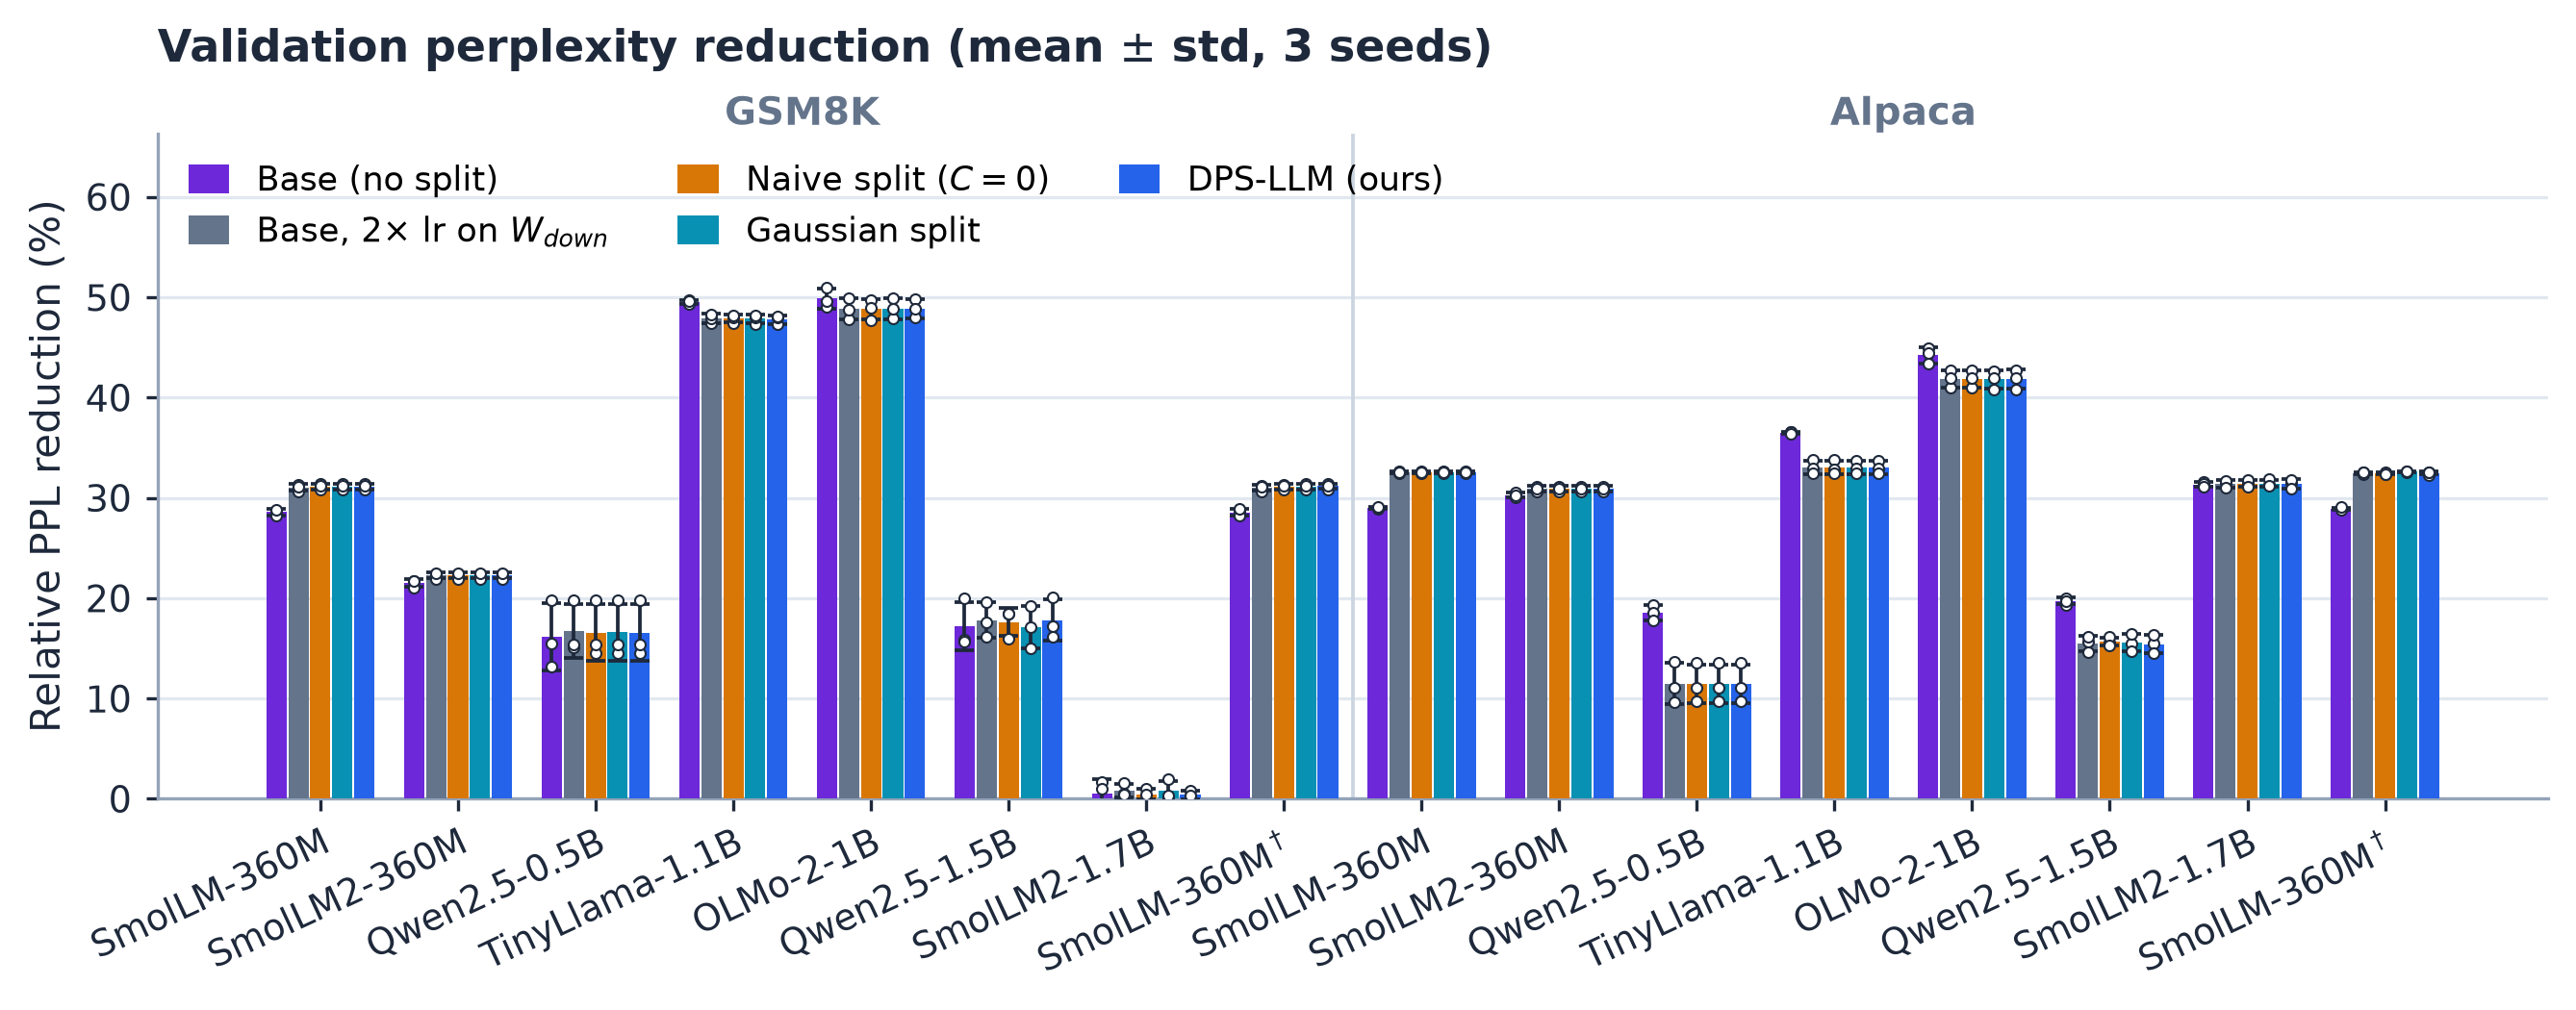
\includegraphics[width=\textwidth]{multi_model_benchmark_comparison.png}
    \caption{\textbf{Benchmark summary}: relative validation-perplexity reduction, mean $\pm$ std over three seeds, with individual seeds as dots. In every setting the three splits (orange, teal, blue) match the matched control (grey), whether they are above or below the unexpanded seed (purple). $^\dagger$: bfloat16 with stochastic rounding.}
    \label{fig:benchmark_results}
\end{figure*}

\subsection{Results}
\label{sec:results}

\paragraph{The split is function-preserving, and the anti-symmetric pairing cancels drift.}
In float32, validation perplexity immediately after the DPS split differs from the seed's by at most $1.3\times10^{-6}$ across all runs, the same as exact duplication ($1.8\times10^{-6}$, from re-associating floating-point sums), whereas Gaussian noise of the same RMS shifts it by up to $2.1\times10^{-4}$. The ablation (Table~\ref{tab:ablation}) shows the same ordering at every noise scale: at $C{=}10^{-1}$ the DPS drift is $1.3\times10^{-3}$ against $1.5\times10^{-2}$ for Gaussian noise, and the anti-symmetric pairing removes the drift that a symmetric $(+\delta,+\delta)$ pairing leaves ($0$ vs.\ $3.0\times10^{-5}$ at $C{=}10^{-4}$), as Proposition~\ref{prop:drift} predicts. Removing the $\tfrac{1}{2}$ factor raises the initial perplexity from 5.13 to 14.47. Under the bfloat16 protocol the split is rounded to nearest, which alone shifts perplexity by up to 0.02.

\paragraph{A split behaves like a learning-rate change.}
In 15 of 18 settings each of the three splits ends within $0.18$ points of the matched control (Table~\ref{tab:empirical_results}, Figure~\ref{fig:benchmark_results}); the exceptions are three noisy GSM8K settings, Qwen2.5-1.5B, SmolLM2-1.7B and Llama-3.2-1B, where the splits are within $0.68$ points of the control and the seed standard deviation is $0.4$--$2.4$. Only one of eighteen DPS-vs-control comparisons reaches $p<0.05$ (SmolLM-360M/GSM8K, $+0.11$ points). Relative to the unexpanded seed at the shared learning rate, splitting looks helpful where the seed is learning-rate-limited (SmolLM-360M: $+2.6$ on GSM8K, $+3.6$ on Alpaca) and harmful where a larger step on $W_{down}$ overshoots (Qwen2.5-0.5B/Alpaca: $-7.1$; Qwen2.5-1.5B/Alpaca: $-4.3$; TinyLlama: $-1.8$ and $-3.5$; OLMo-2-1B: $-1.0$ and $-2.4$; Llama-3.2-1B: $-5.6$ and $-6.0$). The control moves by the same amounts in every case ($+2.5$, $+3.5$, $-7.1$, $-4.2$, $-1.7$, $-3.4$, $-1.0$, $-2.3$, $-5.6$, $-6.1$), so these differences are the step-size effect of Proposition~\ref{prop:lr}, not capacity.

\paragraph{The perturbation does not break the symmetry.}
In float32 the relative distance between paired neurons after 100 steps equals its value at the split to three significant digits ($5.84\times10^{-5}$ for DPS-LLM and $4.13\times10^{-5}$ for Gaussian noise on SmolLM-360M; Figure~\ref{fig:divergence}a), and exactly zero for naive duplication. Across the ablation the distance scales linearly with $C$ and never grows, and the final perplexity is identical to four significant digits for DPS-LLM at every $C\le10^{-2}$ and for Gaussian noise up to $C{=}10^{-3}$ (Table~\ref{tab:ablation}). This is consistent with Proposition~\ref{prop:lr}: a perturbation of relative size $C$ changes the two copies' gradients by $O(C)$, so Adam, whose update depends on the gradient's direction rather than its scale, moves both copies by almost the same step and the initial gap is preserved rather than amplified. Under the bfloat16 protocol, stochastic rounding of each update pulls the copies apart by itself, so even naive duplication reaches a distance of $3.6\times10^{-3}$ on SmolLM-360M (Figure~\ref{fig:divergence}b) and $5$--$12\times10^{-3}$, 64--89\% of the DPS-LLM distance, on the five models of 1B parameters and more; this still yields no consistent gain. Of the fifty-four pairwise comparisons among the three splits only one reaches $p<0.05$ (Gaussian over naive on SmolLM-360M$^\dagger$/Alpaca, $+0.21$ points), fewer than the 2.7 expected by chance.

\paragraph{At matched learning rates the larger model does not win.}
Table~\ref{tab:lr} compares each model's best learning rate for the seed and for DPS-LLM. The differences range from $-3.11$ to $+2.61$ points; the seed is ahead on six of nine settings. The two largest differences come from the largest models. On Qwen2.5-1.5B, DPS-LLM peaks at a lower rate than the seed and diverges at $10^{-4}$ ($-15.6\%$ against $+3.6\%$ for the seed), and on Llama-3.2-1B it degrades much faster than the seed at high rates ($-50.2\%$ against $-15.8\%$ at $10^{-4}$), as expected if the split doubles the effective step on $W_{down}$; on SmolLM2-1.7B both peak at the largest rate swept, so the sweep does not bracket its optimum. Within this budget, the 54--75\% of added parameters do not translate into a consistently lower perplexity.

\paragraph{Accuracy.}
GSM8K exact match on 50 problems is a coarse measure (Table~\ref{tab:accuracy}), but it shows the same pattern. Fine-tuning on reference solutions lowers the accuracy of Qwen2.5-0.5B from 22\% to 9.3\% for the seed and 4.7--5.3\% for the splits and the control, of OLMo-2-1B from 54\% to 16.0\% and 6.7--8.7\%, and of Llama-3.2-1B from 12\% to 3.3\% and 2.7--6.0\%. In all three, the splits stay within 2.6 points (fewer than two problems) of the control, consistent with a larger effective step on $W_{down}$ rather than with the split. The two largest models instead improve: Qwen2.5-1.5B from 12\% to 14.0--17.3\% and SmolLM2-1.7B from 14\% to 32.0--34.0\%, the latter while its GSM8K perplexity falls by less than 1\%, which suggests it mainly learns the answer format; in both, all five conditions lie within 3.3 points, fewer than two of the 50 problems.

\paragraph{Pilot in pure bfloat16.}
With round-to-nearest bfloat16, the $C{=}10^{-4}$ perturbation is absorbed by rounding: the two copies of every neuron kept a cosine similarity of $1.0000$ for 200 steps, and DPS-LLM, Gaussian noise and duplication were statistically indistinguishable ($p\ge0.09$). An emulation of bfloat16 rounding on $\mathcal{N}(0,0.02^2)$ weights shows why: at $C{=}10^{-4}$ the copies differ in only 0.6\% of entries, against 42\% at $C{=}10^{-2}$. The same run also lost most small updates, since an update of $2\times10^{-5}$ is below half a bfloat16 ulp for most weights; SmolLM-360M's base model improved perplexity by 5.3\% in that run despite twice as many steps, against 28.6\% in float32 here.

\begin{figure}[t]
    \centering
    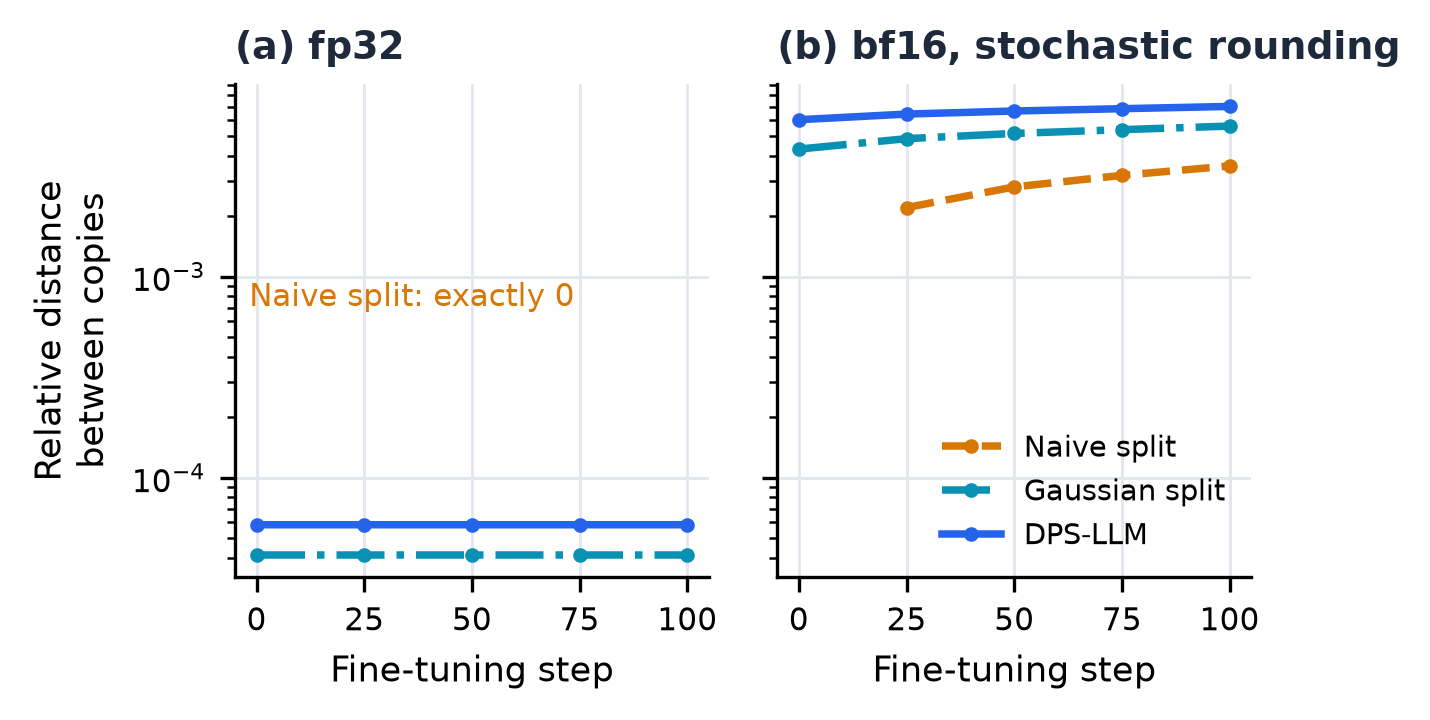
\includegraphics[width=\figwidth]{pair_divergence.png}
    \caption{\textbf{Distance between the two copies of each split neuron} during fine-tuning of SmolLM-360M, mean over seeds and datasets. In float32 (a) the gap created by the perturbation is preserved but never grows. Under bfloat16 with stochastic rounding (b) the rounding itself separates the copies, including for exact duplication.}
    \label{fig:divergence}
\end{figure}

\begin{table}[t]
\centering
\footnotesize
\setlength{\tabcolsep}{4pt}
\caption{\textbf{Best learning rate per model} (GSM8K, seed 42; sweep over $\{1,2,5,10\}\times10^{-5}$): relative perplexity reduction (\%) of the seed and of DPS-LLM, each at its own best rate.}
\label{tab:lr}
\begin{adjustbox}{max width=\columnwidth}\begin{tabular}{@{}lccccc@{}}
\toprule
\textbf{Model} & \multicolumn{2}{c}{\textbf{Base}} & \multicolumn{2}{c}{\textbf{DPS-LLM}} & $\Delta$ \\
\cmidrule(lr){2-3}\cmidrule(lr){4-5}
 & lr & red. & lr & red. & \\
\midrule
SmolLM-360M & $10^{-4}$ & 34.40 & $10^{-4}$ & 34.54 & +0.14 \\
SmolLM2-360M & $5{\times}10^{-5}$ & 23.04 & $5{\times}10^{-5}$ & 22.83 & $-$0.20 \\
Qwen2.5-0.5B & $2{\times}10^{-5}$ & 15.45 & $10^{-5}$ & 15.07 & $-$0.38 \\
TinyLlama-1.1B$^\dagger$ & $10^{-5}$ & 51.45 & $10^{-5}$ & 50.59 & $-$0.87 \\
Llama-3.2-1B$^\dagger$ & $10^{-5}$ & 36.28 & $10^{-5}$ & 34.98 & $-$1.30 \\
OLMo-2-1B$^\dagger$ & $10^{-5}$ & 52.04 & $10^{-5}$ & 51.83 & $-$0.21 \\
Qwen2.5-1.5B$^\dagger$ & $5{\times}10^{-5}$ & 20.60 & $10^{-5}$ & 17.49 & $-$3.11 \\
SmolLM2-1.7B$^\dagger$ & $10^{-4}$ & 7.37 & $10^{-4}$ & 9.98 & +2.61 \\
SmolLM-360M$^\dagger$ & $10^{-4}$ & 34.37 & $10^{-4}$ & 34.57 & +0.19 \\
\bottomrule
\end{tabular}
\end{adjustbox}
\end{table}

\begin{table}[t]
\centering
\footnotesize
\setlength{\tabcolsep}{4pt}
\caption{\textbf{GSM8K exact-match accuracy (\%)} on 50 test problems before fine-tuning and after it (mean over seeds).}
\label{tab:accuracy}
\begin{adjustbox}{max width=\columnwidth}\begin{tabular}{@{}lcccccc@{}}
\toprule
\textbf{Model} & \textbf{Before} & \textbf{Base} & \textbf{2$\times$ ctrl} & \textbf{Naive} & \textbf{Gauss.} & \textbf{DPS} \\
\midrule
SmolLM-360M & 2 & 0.7 & 3.3 & 4.0 & 4.0 & 4.0 \\
SmolLM2-360M & 0 & 5.3 & 7.3 & 8.0 & 7.3 & 8.0 \\
Qwen2.5-0.5B & 22 & 9.3 & 5.3 & 4.7 & 4.7 & 4.7 \\
TinyLlama-1.1B$^\dagger$ & 0 & 2.0 & 2.7 & 2.0 & 4.0 & 0.7 \\
OLMo-2-1B$^\dagger$ & 54 & 16.0 & 7.3 & 8.7 & 6.7 & 7.3 \\
SmolLM-360M$^\dagger$ & 2 & 2.7 & 2.0 & 3.3 & 2.0 & 2.0 \\
\bottomrule
\end{tabular}
\end{adjustbox}
\end{table}

\begin{table}[t]
\centering
\footnotesize
\setlength{\tabcolsep}{3pt}
\caption{\textbf{Ablations} on SmolLM-360M/GSM8K, float32, seed 42, 50 steps. \emph{Init drift}: change of validation perplexity caused by the split (base: 5.13). \emph{Red.}: relative perplexity reduction after fine-tuning. \emph{Pair dist.}: relative distance between paired neurons after fine-tuning.}
\label{tab:ablation}
\begin{adjustbox}{max width=\columnwidth}\begin{tabular}{@{}lccc@{}}
\toprule
\textbf{Variant} & \textbf{Init drift} & \textbf{Red.\ (\%)} & \textbf{Pair dist.} \\
\midrule
Base (no split) & 0 & 22.31 & -- \\
Naive split & 0 & 25.78 & 0 \\
\midrule
DPS, $C{=}10^{-5}$ & 0 & 25.78 & $5.8{\times}10^{-6}$ \\
Gaussian, $C{=}10^{-5}$ & $+6.2{\times}10^{-7}$ & 25.78 & $4.1{\times}10^{-6}$ \\
DPS, $C{=}10^{-4}$ & 0 & 25.78 & $5.8{\times}10^{-5}$ \\
Gaussian, $C{=}10^{-4}$ & $+3.2{\times}10^{-6}$ & 25.78 & $4.1{\times}10^{-5}$ \\
DPS, $C{=}10^{-3}$ & $+5.1{\times}10^{-7}$ & 25.78 & $5.8{\times}10^{-4}$ \\
Gaussian, $C{=}10^{-3}$ & $+2.5{\times}10^{-5}$ & 25.78 & $4.1{\times}10^{-4}$ \\
DPS, $C{=}10^{-2}$ & $+1.4{\times}10^{-5}$ & 25.78 & $5.8{\times}10^{-3}$ \\
Gaussian, $C{=}10^{-2}$ & $+3.5{\times}10^{-4}$ & 25.75 & $4.1{\times}10^{-3}$ \\
DPS, $C{=}10^{-1}$ & $+1.3{\times}10^{-3}$ & 25.80 & $5.8{\times}10^{-2}$ \\
Gaussian, $C{=}10^{-1}$ & $+1.5{\times}10^{-2}$ & 25.55 & $4.1{\times}10^{-2}$ \\
\midrule
DPS, symmetric $(+\delta,+\delta)$ & $+3.0{\times}10^{-5}$ & 25.78 & 0 \\
DPS, no $\tfrac{1}{2}$ factor & +9.34 & 60.52 & $5.8{\times}10^{-5}$ \\
\bottomrule
\end{tabular}
\end{adjustbox}
\end{table}

% -----------------------------------------------------------------------------
\section{Conclusion}
The function-preserving half of DPS-LLM works as designed: placing the factor $\tfrac{1}{2}$ on the down projection grows the SwiGLU blocks of a pre-trained LLM without changing its output, and the anti-symmetric, polarity-signed perturbation cancels first-order drift in practice, by two orders of magnitude relative to Gaussian noise. The symmetry-breaking half does not take effect during fine-tuning: the gap between paired neurons is preserved but never amplified, so the split model behaves like its seed, and under Adam that means like its seed with a doubled learning rate on $W_{down}$. A matched control reproduces every gain and loss we observe, and at each model's best learning rate the split model is not consistently better than the seed. We draw two lessons for work on model growth. Comparisons of a grown model with its seed at a shared learning rate conflate capacity with step size and need the matched control; and symmetry breaking should be verified by measuring whether the copies diverge, not assumed from the perturbation. Whether larger noise, longer training from scratch-scale budgets, or growth during pre-training changes this picture remains open; the same operator applies to MoE upcycling and LoRA rank growth, which we have not evaluated.

% -----------------------------------------------------------------------------
\section*{Limitations}
\textbf{Scale.} We evaluate eight models up to 1.7B parameters, fine-tuned for 50 optimiser updates on 256 examples; capacity effects may only appear with larger models, larger datasets or longer training, and in pre-training rather than fine-tuning.
\textbf{Statistics.} Three seeds per condition detect only differences of a few tenths of a point; the learning-rate sweep and the ablations use a single seed, and the sweep does not bracket the best rate of SmolLM2-1.7B.
\textbf{Precision.} The five models of 1B parameters and more use bfloat16 with stochastic rounding and a larger noise scale than the float32 models, so their noise condition is not identical; on SmolLM-360M the two protocols agree within $0.2$ points for every condition.
\textbf{Scope.} Only width splitting of the MLP was evaluated, with only the MLP parameters trainable; depth growth, attention-head splitting, the MoE and LoRA regimes, and full-parameter fine-tuning are untested. We measure perplexity and GSM8K exact match but not instruction-following quality for Alpaca-Cleaned.
\textbf{Data provenance.} The Alpaca-Cleaned validation examples come from its training split; they are unseen during our fine-tuning but may have been seen during the checkpoints' original training.

\section*{\ethicsheading}
This work modifies the architecture of publicly released language models and uses two public datasets (GSM8K, MIT licence; Alpaca-Cleaned, CC~BY-NC~4.0) and eight public checkpoints (Qwen2.5-0.5B-Instruct, Qwen2.5-1.5B-Instruct, SmolLM-360M-Instruct, SmolLM2-360M-Instruct, SmolLM2-1.7B-Instruct, TinyLlama-1.1B-Chat and OLMo-2-0425-1B-Instruct, all Apache~2.0; Llama-3.2-1B-Instruct, Llama~3.2 Community License, used under its terms for research). Growing a model does not change the biases or safety properties of its seed, and a grown model inherits any limitations of the original checkpoint; practitioners should re-run their safety evaluations after expansion. All experiments ran on a free cloud GPU tier with a small compute footprint (about 23 hours on a two-T4 instance for the benchmark, sweeps and ablations, and 4 for the pilot). No human subjects or personal data were involved.

\ifdefined\FINAL\def\showacknowledgements{}\fi
\ifdefined\ARXIV\def\showacknowledgements{}\fi
\ifdefined\showacknowledgements
\section*{Acknowledgements}
The author thanks Dr.~M.~Ali Tahir (SEECS, National University of Sciences and Technology) for supervising the thesis on which this work builds.
\fi
:
\providecommand{\figwidth}{\columnwidth}          % width of single-column figures
\providecommand{\appref}[1]{Appendix~\ref{#1}}   % IJCAI: appendix is supplementary
\providecommand{\ethicsheading}{Ethics Statement} % ICML: Impact Statement

\begin{abstract}
Growing a pre-trained large language model (LLM) in place, instead of training a larger one from scratch, needs an expansion that preserves the model's function and a way to make the added parameters useful.
We study \textbf{Discriminative Parameter Splitting for LLMs (DPS-LLM)}, which doubles the intermediate width of every SwiGLU feed-forward block by duplicating the gate and up projections and the $\tfrac{1}{2}$-scaled down projection, and breaks the symmetry of the copies with a polarity-preserving, anti-symmetric perturbation adapted from LSTM acoustic models.
We prove that the split is exactly function-preserving and that the anti-symmetric pairing cancels first-order output drift, and confirm both on eight open-weight models from 360M to 1.7B parameters: in float32, the DPS split changes validation perplexity by at most $1.3\times10^{-6}$, two orders of magnitude less than Gaussian noise of the same size.
Its effect on fine-tuning is not what growth methods assume. We prove that under Adam an exact split trains like its seed with a doubled learning rate on the down projection, and a matched control, the unexpanded model with that learning rate, reproduces the split's perplexity reduction on every model and dataset, within $0.18$ points in 15 of 18 settings and within seed noise in the other three.
The perturbation does not break the symmetry: in float32 the distance between paired neurons stays constant during fine-tuning, and DPS-LLM, Gaussian noise and exact duplication are statistically indistinguishable. At each model's best learning rate, the split model, 54--75\% larger, is ahead of its seed on only three of nine settings.
We release code, notebooks and all per-seed results, and argue that evaluations of model growth need matched learning-rate controls.
\end{abstract}

% -----------------------------------------------------------------------------
\section{Introduction}
Transformer LLMs \citep{vaswani2017attention,touvron2023llama,qwen2024technical} are almost always trained under a \emph{static} paradigm: every dimension of the network is fixed \textit{a priori}, the weights are drawn from a random initialization \citep{glorot2010understanding,he2015delving}, and the model is trained end-to-end.
Scaling laws \citep{kaplan2020scaling,hoffmann2022chinchilla} make the cost of this paradigm explicit: a larger model must be trained from scratch, spending much of its early budget on features a smaller model already possesses.
The same rigidity appears at fine-tuning time. When a compact model saturates its parametric capacity on a domain-specific task, practitioners must either accept the plateau or restart with a larger architecture.

Progressive growth offers an alternative: begin with a compact \emph{seed} model and enlarge it during training \citep{chen2015net2net,gong2019stacking,chen2022bert2bert,wang2023ligo}.
Two requirements make growth practical for modern LLMs.
First, the expansion must be \emph{function-preserving}, so that the grown model neither loses the seed's knowledge nor suffers a loss spike.
Second, the duplicated parameters must be \emph{distinguishable}; otherwise identical copies receive identical gradients and the added capacity is never used \citep{chen2015net2net}.
Existing work on Transformers has addressed these requirements for pre-LayerNorm blocks with ReLU or GELU feed-forward layers \citep{chen2022bert2bert,wang2024lemon}, but gated SwiGLU blocks \citep{shazeer2020glu}, which are now standard in LLaMA, Mistral, Gemma, Qwen and SmolLM, multiply two projections element-wise, so naive duplication doubles the block's output.

We adapt \emph{Discriminative Parameter Splitting} \citep{irfan2021discriminative}, originally developed for growing LSTM acoustic models, to SwiGLU Transformers, and ask whether it delivers on both requirements when a pre-trained LLM is fine-tuned. Our contributions are:
\begin{itemize}
    \item \textbf{An exact function-preserving SwiGLU split with drift-cancelling noise.} Duplicating the rows of $W_{gate}$ and $W_{up}$ and the columns of $\tfrac{1}{2}W_{down}$ doubles $d_{ffn}$ with provably identical output (Theorem~\ref{thm:invariance}), and a polarity-signed, anti-symmetric perturbation cancels first-order drift (Proposition~\ref{prop:drift}). Both hold on real checkpoints.
    \item \textbf{A split is a learning-rate change.} Under Adam, an exact split trains like its seed with a doubled learning rate on $W_{down}$ (Proposition~\ref{prop:lr}). We introduce the matched control this implies and show that it reproduces the split's gains.
    \item \textbf{A controlled benchmark.} On eight open-weight models from four families (360M--1.7B), two datasets, five conditions, three seeds, per-model learning-rate sweeps and ablations, we find no gain from added capacity and no symmetry breaking during fine-tuning.
    \item \textbf{A precision pitfall.} In bfloat16 the default perturbation is rounded away entirely; we give a stochastic-rounding protocol under which it survives.
\end{itemize}
We also describe, and release code for, two further regimes of the same operator---dense-to-Mixture-of-Experts (MoE) upcycling and LoRA rank doubling---which we leave for empirical evaluation in future work (\appref{app:regimes}).

\begin{figure}[t]
    \centering
    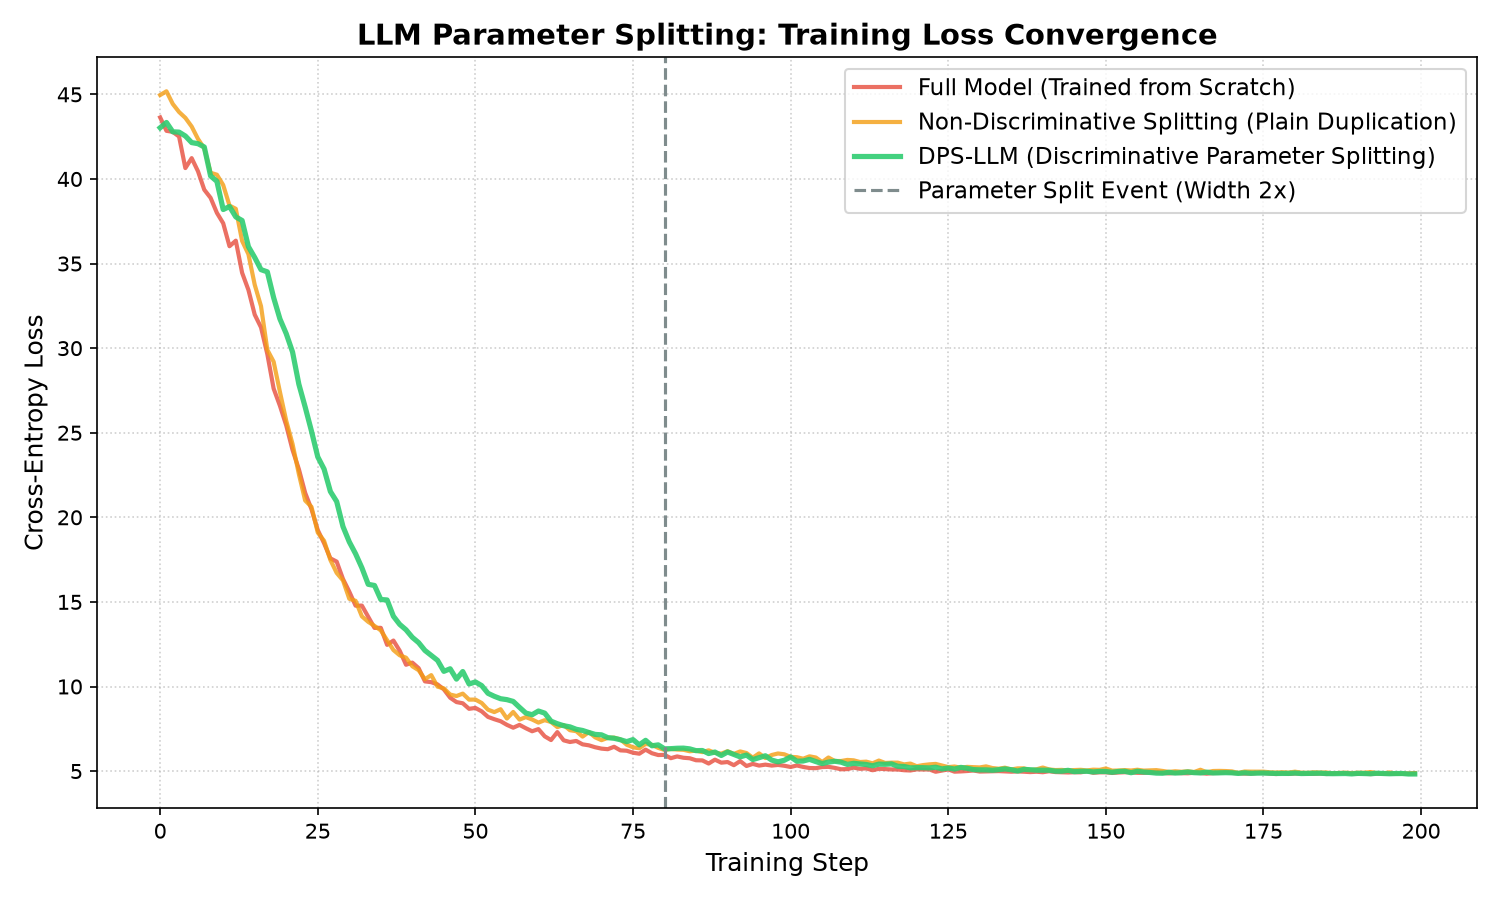
\includegraphics[width=\figwidth]{dps_llm_training_curve.png}
    \caption{\textbf{Controlled split on a synthetic language-modelling task.} A two-layer SwiGLU Transformer with $d_{ffn}=64$ is trained for 80 steps and then split to $d_{ffn}=128$ (dashed line). Both split variants continue without a loss spike, whereas the $d_{ffn}=128$ model trained from scratch spends its first 80 steps re-learning what the seed already knows. DPS-LLM and plain duplication converge to the same loss as the full model by step 200.}
    \label{fig:training_curve}
\end{figure}

% -----------------------------------------------------------------------------
\section{Related Work}
\paragraph{Function-preserving growth.}
Net2Net \citep{chen2015net2net} introduced \emph{Net2WiderNet} and \emph{Net2DeeperNet}, which widen or deepen a network without changing its function, and noted that a small amount of noise is needed to break the symmetry of copied units. Network morphism \citep{wei2016morphism} generalised the idea to arbitrary non-linear morphisms.
For Transformers, progressive stacking \citep{gong2019stacking} and staged training \citep{shen2022staged} grow depth and width of BERT-style encoders; bert2BERT \citep{chen2022bert2bert} extends Net2Net to attention blocks with function-preserving and advanced knowledge initialisation; LiGO \citep{wang2023ligo} learns a linear growth operator from the small model; MSG \citep{yao2024msg} and LEMON \citep{wang2024lemon} obtain lossless expansion for pre-LayerNorm blocks by masking or by an explicit average-and-cancel construction.
Depth up-scaling \citep{kim2024solar} and HyperCloning \citep{samragh2024hypercloning} apply the same principle to decoder-only LLMs, the latter by tiling weights of a small model into a wider one.
DPS-LLM belongs to this family but targets the gated SwiGLU block specifically, where the $\tfrac{1}{2}$ factor must be placed on the down projection to preserve function.

\paragraph{Neuron splitting.}
Splitting steepest descent \citep{liu2019splitting}, Firefly descent \citep{wu2020firefly} and GradMax \citep{evci2022gradmax} choose \emph{which} neurons to split and \emph{how} to perturb the copies using second-order or gradient information. These methods are principled but require extra computation per split; DPS-LLM instead splits every neuron and uses a closed-form, gradient-free perturbation whose only statistic is the standard deviation of the weight matrix.

\paragraph{Mixture-of-Experts upcycling.}
Sparse upcycling \citep{komatsuzaki2022sparse} initialises MoE experts \citep{shazeer2017outrageously,lepikhin2021gshard,fedus2022switch} by cloning a dense MLP, and \citet{he2024upcycling} study this recipe at scale; Mixtral \citep{jiang2024mixtral} is a widely used dense-to-sparse architecture. Cloned experts are initially identical, so the same symmetry problem arises; our anti-symmetric noise is directly applicable (\appref{app:regimes}).

\paragraph{Adapter rank growth.}
LoRA \citep{hu2021lora} fixes the adapter rank in advance; AdaLoRA \citep{zhang2023adalora} and DyLoRA \citep{valipour2023dylora} adapt the rank during training. Rank doubling by parameter splitting (\appref{app:regimes}) is a complementary, function-preserving way to increase adapter capacity.

\paragraph{Discriminative splitting in speech.}
\citet{irfan2021discriminative} grew LSTM-RNN acoustic models by duplicating rows and columns of weight matrices and injecting a polarity-preserving perturbation, reporting faster convergence, less over-training and a 1.2\% absolute word-error-rate reduction over Xavier initialisation on a Kaldi/VoxForge recipe. This paper transfers that recipe to Transformers and adds the invariance scaling and the anti-symmetric pairing.

% -----------------------------------------------------------------------------
\section{Method}
\subsection{Function-preserving SwiGLU width splitting}
\label{sec:split}
Modern decoder blocks \citep{shazeer2020glu,touvron2023llama,qwen2024technical} use a gated feed-forward network
\begin{equation}
    \mathrm{FFN}(x) = W_{down}\,\big(\mathrm{SiLU}(W_{gate}x) \odot W_{up}x\big),
    \label{eq:swiglu}
\end{equation}
with $W_{gate},W_{up}\in\mathbb{R}^{d_{ffn}\times d_{model}}$, $W_{down}\in\mathbb{R}^{d_{model}\times d_{ffn}}$, and $\mathrm{SiLU}(z)=z\,\sigma(z)$ \citep{hendrycks2016gelu,elfwing2018silu,ramachandran2017swish}. Let $h(x)=\mathrm{SiLU}(W_{gate}x)\odot W_{up}x\in\mathbb{R}^{d_{ffn}}$.

To grow $d_{ffn}\to 2d_{ffn}$ we apply \emph{rows extension} to the two incoming projections and \emph{columns extension} with a $\tfrac{1}{2}$ factor to the outgoing projection:
\begin{align}
    W_{gate}^{\prime} &= \begin{bmatrix} W_{gate}+\Delta_{gate}^{(1)} \\ W_{gate}+\Delta_{gate}^{(2)} \end{bmatrix}, \label{eq:rows}\\
    W_{up}^{\prime} &= \begin{bmatrix} W_{up}+\Delta_{up}^{(1)} \\ W_{up}+\Delta_{up}^{(2)} \end{bmatrix}, \label{eq:rows_up}\\
    W_{down}^{\prime} &= \tfrac{1}{2}\begin{bmatrix} W_{down} & W_{down} \end{bmatrix} \nonumber\\
    &\quad + \begin{bmatrix} \Delta_{down}^{(1)} & \Delta_{down}^{(2)} \end{bmatrix}. \label{eq:cols}
\end{align}

\begin{theorem}[Functional invariance]
\label{thm:invariance}
With $\Delta=0$, $\mathrm{FFN}'(x)=\mathrm{FFN}(x)$ for every input $x$.
\end{theorem}
\begin{proof}
The stacked gate and up projections produce $[h(x);\,h(x)]$, so
$\mathrm{FFN}'(x)=\tfrac{1}{2}W_{down}h(x)+\tfrac{1}{2}W_{down}h(x)=W_{down}h(x)$.
\end{proof}
Because every block is invariant and the residual stream, attention and normalisation layers are untouched, the whole model is invariant; the loss on any batch is unchanged in exact arithmetic. Without the $\tfrac{1}{2}$ factor the block's output would double, which is the loss spike observed when SwiGLU networks are naively widened.

\subsection{Calculated Anti-Symmetric Noise}
\label{sec:noise}
If $\Delta=0$, the two copies of every neuron are identical and receive identical gradients for the rest of training, so the expanded model has no more effective capacity than the seed \citep{chen2015net2net}.
Isotropic Gaussian noise breaks the tie but is sign-agnostic: it flips the polarity of small weights, which \citet{irfan2021discriminative} found harmful for pre-trained LSTMs.
We instead use a perturbation whose sign is dictated by the weight it perturbs. For a weight matrix $W$ with element-wise standard deviation $\sigma_W$, draw $u\sim\mathcal{U}(0,1)$ and $n\sim\mathcal{N}(0,1)$ independently per element and set
\begin{align}
    f(W) &= \big|(u-\tfrac{1}{2})\cdot C\,\sigma_W\cdot n\big|, \label{eq:f}\\
    \delta(W) &= \mathrm{sign}(W)\odot f(W), \label{eq:delta}\\
    \Delta^{(1)} &= +\delta(W), \qquad \Delta^{(2)} = -\delta(W). \label{eq:pair}
\end{align}
The modulation constant $C=10^{-4}$ is inherited from the original speech recipe; \eqref{eq:f}--\eqref{eq:delta} are its Equations 5.7--5.8 with the noise scaled by $\sigma_W$ so that the same $C$ transfers across layers of different magnitude. Equation~\eqref{eq:pair} is new: the two copies receive \emph{opposite} perturbations. For $W_{down}$ the noise is computed on the already-halved matrix.

\begin{proposition}[Sign preservation]
\label{prop:sign}
Copy 1 satisfies $|w+\delta(w)|=|w|+f(w)>|w|$ for every weight, so no sign is flipped. Copy 2 satisfies $|w-\delta(w)|=\big||w|-f(w)\big|$ and flips sign only if $|w|<f(w)$.
\end{proposition}
Since $f(w)\leq\tfrac{1}{2}C\sigma_W|n|$, a flip requires $|w|<\tfrac{1}{2}\cdot10^{-4}\sigma_W|n|$; for approximately Gaussian weights this is a fraction on the order of $10^{-4}$ of the matrix or less, and these weights carry negligible signal. In our runs the measured sign-flip fraction is $8$--$9\times10^{-6}$ (Section~\ref{sec:results}).

\begin{proposition}[First-order drift cancellation]
\label{prop:drift}
With the pairing in \eqref{eq:pair}, $\mathrm{FFN}'(x)=\mathrm{FFN}(x)+O(\|\delta\|^2)$.
\end{proposition}
\begin{proof}
Write $h_{1}(x)$ and $h_{2}(x)$ for the hidden activations of the two copies. A first-order expansion in $\delta$ gives $h_{1}=h+J\delta x+O(\delta^2)$ and $h_{2}=h-J\delta x+O(\delta^2)$ for the same Jacobian $J$, so $\tfrac{1}{2}W_{down}(h_{1}+h_{2})=W_{down}h+O(\delta^2)$. The down-projection perturbation contributes $\delta_{down}h_{1}-\delta_{down}h_{2}=\delta_{down}(h_{1}-h_{2})=O(\delta^2)$.
\end{proof}
The perturbation therefore does two things at once: it leaves the output unchanged to first order, and it makes $\nabla_{W^{(1)}}\mathcal{L}\neq\nabla_{W^{(2)}}\mathcal{L}$ from the very first update, because the two copies now see different pre-activations. Both statements assume that the perturbation is representable in the weight format. bfloat16 keeps 8 significant bits, so a perturbation of relative size $10^{-4}$ is rounded away for all but the smallest weights; Section~\ref{sec:results} shows that this is what happens in practice.

\subsection{An exact split changes the effective learning rate}
\label{sec:lr_equiv}
Function preservation holds at the moment of the split, but not along the optimisation trajectory. With Adam-type optimisers \citep{kingma2015adam,loshchilov2019adamw}, the split also changes the effective step size of the block.
\begin{proposition}[Split as learning-rate doubling]
\label{prop:lr}
Let the split be exact ($\Delta=0$) and let both models be trained with Adam at learning rate $\eta$. Then, up to Adam's $\epsilon$, the copies stay identical and the split model follows the trajectory of the unsplit model trained with learning rate $\eta$ on $W_{gate},W_{up}$ and $2\eta$ on $W_{down}$.
\end{proposition}
\begin{proof}[Proof sketch]
While the copies are identical, each copy of a row of $W_{gate}$ or $W_{up}$ receives exactly half the gradient of the original row, because it feeds a down-projection column scaled by $\tfrac{1}{2}$; Adam's update is invariant to a constant rescaling of the gradient, so both copies take the step the original would take, and stay identical. Each copy of a column of $W_{down}$ receives the full gradient of the original column, because it sees the same activation; both copies take the original's step, and the effective matrix $W^{(1)}_{down}+W^{(2)}_{down}$ moves twice as far.
\end{proof}
The equivalence is exact in exact arithmetic without gradient clipping and with decoupled weight decay ignored; global-norm clipping, which rescales all gradients jointly, and finite precision make it approximate. On a toy SwiGLU block trained with AdamW in float32 for 100 steps, the losses of the exact split and of the unsplit block with a $2\times$ learning rate on $W_{down}$ differ by at most $7\times10^{-6}$, against $2.4\times10^{-2}$ from the unsplit block at the original learning rate. Comparisons between a split model and its seed at one shared learning rate therefore conflate added capacity with a larger step on $W_{down}$; Section~\ref{sec:results} confirms the equivalence on real checkpoints.

\subsection{Applying the operator to a pre-trained LLM}
The split is applied in place to every decoder layer of a Hugging Face checkpoint \citep{wolf2020transformers}: the three linear layers are replaced by their expanded versions and \texttt{intermediate\_size} is doubled in the configuration. No other tensors change. For Qwen2.5-0.5B this grows $d_{ffn}$ from 4864 to 9728 in all 24 layers (+313.8M parameters); for SmolLM-360M from 2560 to 5120 in all 32 layers (+236.0M).

% -----------------------------------------------------------------------------
\begin{table*}[t]
\centering
\small
\setlength{\tabcolsep}{3pt}
\caption{\textbf{Relative validation-perplexity reduction (\%) after fine-tuning}, mean{\scriptsize$\pm$std} over three seeds (higher is better; bold: best mean per row). \emph{Base, 2$\times$ lr $W_{down}$} is the unexpanded model trained with a doubled learning rate on the down projection, the matched control of Proposition~\ref{prop:lr}. \emph{DPS $-$ ctrl}: mean paired difference between DPS-LLM and the control, with the paired $t$-test $p$-value. Models without a mark are fine-tuned in float32 with $C{=}10^{-4}$; $^\dagger$: bfloat16 with stochastic rounding and $C{=}10^{-2}$.}
\label{tab:empirical_results}
\vspace{2pt}
\begin{adjustbox}{max width=\textwidth}\begin{tabular}{@{}llcccccc@{}}
\toprule
\textbf{Model} & \textbf{Data} & \textbf{Base} & \textbf{Base, 2$\times$ lr $W_{down}$} & \textbf{Naive split} & \textbf{Gaussian split} & \textbf{DPS-LLM} & \textbf{DPS $-$ ctrl ($p$)} \\
\midrule
SmolLM-360M & GSM8K & 28.58{\scriptsize$\pm$0.30} & 31.04{\scriptsize$\pm$0.32} & \textbf{31.15{\scriptsize$\pm$0.30}} & \textbf{31.15{\scriptsize$\pm$0.30}} & \textbf{31.15{\scriptsize$\pm$0.30}} & +0.11 (0.04) \\
SmolLM2-360M & GSM8K & 21.51{\scriptsize$\pm$0.39} & 22.28{\scriptsize$\pm$0.32} & \textbf{22.29{\scriptsize$\pm$0.32}} & \textbf{22.29{\scriptsize$\pm$0.32}} & \textbf{22.29{\scriptsize$\pm$0.32}} & +0.01 (0.12) \\
Qwen2.5-0.5B & GSM8K & 16.12{\scriptsize$\pm$3.35} & \textbf{16.75{\scriptsize$\pm$2.66}} & 16.58{\scriptsize$\pm$2.86} & 16.60{\scriptsize$\pm$2.83} & 16.58{\scriptsize$\pm$2.86} & $-$0.17 (0.50) \\
TinyLlama-1.1B$^\dagger$ & GSM8K & \textbf{49.55{\scriptsize$\pm$0.21}} & 47.88{\scriptsize$\pm$0.45} & 47.86{\scriptsize$\pm$0.38} & 47.85{\scriptsize$\pm$0.46} & 47.79{\scriptsize$\pm$0.43} & $-$0.09 (0.41) \\
Llama-3.2-1B$^\dagger$ & GSM8K & \textbf{31.95{\scriptsize$\pm$0.96}} & 26.34{\scriptsize$\pm$2.08} & 26.80{\scriptsize$\pm$1.55} & 26.59{\scriptsize$\pm$2.02} & 26.37{\scriptsize$\pm$2.02} & +0.03 (0.74) \\
OLMo-2-1B$^\dagger$ & GSM8K & \textbf{49.88{\scriptsize$\pm$1.00}} & 48.83{\scriptsize$\pm$1.04} & 48.82{\scriptsize$\pm$1.00} & 48.85{\scriptsize$\pm$1.01} & 48.89{\scriptsize$\pm$0.95} & +0.06 (0.39) \\
Qwen2.5-1.5B$^\dagger$ & GSM8K & 17.20{\scriptsize$\pm$2.41} & 17.79{\scriptsize$\pm$1.77} & 17.62{\scriptsize$\pm$1.40} & 17.12{\scriptsize$\pm$2.10} & \textbf{17.83{\scriptsize$\pm$2.03}} & +0.03 (0.90) \\
SmolLM2-1.7B$^\dagger$ & GSM8K & 0.55{\scriptsize$\pm$1.41} & \textbf{0.82{\scriptsize$\pm$0.67}} & 0.46{\scriptsize$\pm$0.55} & 0.79{\scriptsize$\pm$0.99} & 0.40{\scriptsize$\pm$0.42} & $-$0.42 (0.19) \\
SmolLM-360M$^\dagger$ & GSM8K & 28.57{\scriptsize$\pm$0.33} & 31.03{\scriptsize$\pm$0.31} & 31.12{\scriptsize$\pm$0.27} & 31.14{\scriptsize$\pm$0.29} & \textbf{31.16{\scriptsize$\pm$0.29}} & +0.13 (0.07) \\
\midrule
SmolLM-360M & Alpaca & 29.02{\scriptsize$\pm$0.08} & 32.55{\scriptsize$\pm$0.10} & \textbf{32.58{\scriptsize$\pm$0.09}} & \textbf{32.58{\scriptsize$\pm$0.09}} & \textbf{32.58{\scriptsize$\pm$0.09}} & +0.03 (0.14) \\
SmolLM2-360M & Alpaca & 30.27{\scriptsize$\pm$0.23} & \textbf{30.91{\scriptsize$\pm$0.28}} & \textbf{30.91{\scriptsize$\pm$0.29}} & \textbf{30.91{\scriptsize$\pm$0.29}} & \textbf{30.91{\scriptsize$\pm$0.29}} & +0.00 (0.62) \\
Qwen2.5-0.5B & Alpaca & \textbf{18.56{\scriptsize$\pm$0.73}} & 11.47{\scriptsize$\pm$2.07} & 11.47{\scriptsize$\pm$1.95} & 11.47{\scriptsize$\pm$1.95} & 11.47{\scriptsize$\pm$1.95} & +0.00 (0.96) \\
TinyLlama-1.1B$^\dagger$ & Alpaca & \textbf{36.51{\scriptsize$\pm$0.08}} & 33.07{\scriptsize$\pm$0.67} & 33.05{\scriptsize$\pm$0.65} & 33.04{\scriptsize$\pm$0.63} & 33.04{\scriptsize$\pm$0.63} & $-$0.03 (0.25) \\
Llama-3.2-1B$^\dagger$ & Alpaca & \textbf{38.36{\scriptsize$\pm$0.09}} & 32.24{\scriptsize$\pm$0.46} & 32.26{\scriptsize$\pm$0.45} & 32.30{\scriptsize$\pm$0.51} & 32.36{\scriptsize$\pm$0.35} & +0.13 (0.30) \\
OLMo-2-1B$^\dagger$ & Alpaca & \textbf{44.22{\scriptsize$\pm$0.79}} & 41.89{\scriptsize$\pm$0.85} & 41.88{\scriptsize$\pm$0.87} & 41.81{\scriptsize$\pm$0.92} & 41.82{\scriptsize$\pm$0.97} & $-$0.07 (0.42) \\
Qwen2.5-1.5B$^\dagger$ & Alpaca & \textbf{19.71{\scriptsize$\pm$0.34}} & 15.50{\scriptsize$\pm$0.78} & 15.68{\scriptsize$\pm$0.40} & 15.54{\scriptsize$\pm$0.87} & 15.43{\scriptsize$\pm$0.88} & $-$0.07 (0.55) \\
SmolLM2-1.7B$^\dagger$ & Alpaca & 31.34{\scriptsize$\pm$0.25} & 31.42{\scriptsize$\pm$0.37} & \textbf{31.45{\scriptsize$\pm$0.37}} & \textbf{31.45{\scriptsize$\pm$0.35}} & 31.41{\scriptsize$\pm$0.45} & $-$0.01 (0.78) \\
SmolLM-360M$^\dagger$ & Alpaca & 28.92{\scriptsize$\pm$0.14} & 32.49{\scriptsize$\pm$0.10} & 32.42{\scriptsize$\pm$0.10} & \textbf{32.63{\scriptsize$\pm$0.06}} & 32.47{\scriptsize$\pm$0.15} & $-$0.02 (0.61) \\
\bottomrule
\end{tabular}
\end{adjustbox}
\end{table*}

\section{Experiments}
\subsection{Setup}
\label{sec:setup}
\paragraph{Models and precision.}
We use eight instruction-tuned open-weight checkpoints with SwiGLU blocks of the form \eqref{eq:swiglu}: SmolLM-360M, SmolLM2-360M and SmolLM2-1.7B \citep{allal2024smollm,allal2025smollm2}, Qwen2.5-0.5B and Qwen2.5-1.5B \citep{qwen2024technical}, TinyLlama-1.1B \citep{zhang2024tinyllama}, Llama-3.2-1B \citep{grattafiori2024llama3}, and OLMo-2-1B \citep{olmo2024olmo2}. The three models below 1B parameters are fine-tuned entirely in float32, where the $C{=}10^{-4}$ perturbation is representable. Models of 1B parameters and more are fine-tuned in bfloat16 to stay within the memory of two 16\,GB GPUs after splitting, with bfloat16 weights, an AdamW update computed in float32 and written back with stochastic rounding \citep{gupta2015deep,zamirai2020revisiting} (so updates smaller than half a unit in the last place are applied in expectation), and $C{=}10^{-2}$, because the split itself is rounded to nearest and a $C{=}10^{-4}$ perturbation would survive in only 0.6\% of entries (Section~\ref{sec:results}). To compare the two protocols on one checkpoint, SmolLM-360M is also run under the bfloat16 protocol (marked $^\dagger$).

\paragraph{Data.}
GSM8K \citep{cobbe2021gsm8k} and Alpaca-Cleaned \citep{taori2023alpaca,yahma2023alpacacleaned}, rendered with fixed templates (\appref{app:prompts}). For GSM8K we fine-tune on 256 examples drawn from the training split and measure perplexity on the first 100 test problems. For Alpaca-Cleaned, which has no test split, a fixed permutation of the training split provides 256 fine-tuning and 100 disjoint validation examples. GSM8K accuracy is exact match of the final number, generated greedily (at most 256 new tokens) for the first 50 test problems, before fine-tuning once per model and after fine-tuning for every run.

\paragraph{Conditions.}
(1) \emph{Base}: the unmodified checkpoint. (2) \emph{Base, 2$\times$ lr $W_{down}$}: the unmodified checkpoint with a doubled learning rate on every down projection, the matched control of Proposition~\ref{prop:lr}. (3) \emph{Naive split}: Eqs.~\eqref{eq:rows}--\eqref{eq:cols} with $\Delta{=}0$. (4) \emph{Gaussian split}: i.i.d.\ Gaussian noise drawn independently for each copy, as in Net2Net \citep{chen2015net2net}, with standard deviation $C\sigma_W/\sqrt{12}$ so that its RMS matches the calculated noise. (5) \emph{DPS-LLM}: Calculated Anti-Symmetric Noise.

\paragraph{Fine-tuning and evaluation.}
All conditions share one recipe (Table~\ref{tab:hparams}); only the SwiGLU parameters are trained, so the comparison isolates the expanded block. Validation perplexity \citep{jelinek1977perplexity} is $\exp$ of the mean per-sequence cross-entropy, measured before the first and after the last update. Every condition is run with seeds 42, 43 and 44, which set the noise draw and the order of the training examples; we report mean$\pm$std and paired $t$-tests across seeds. Every 25 steps we record the mean relative distance $\|a-b\|/\tfrac{1}{2}(\|a\|+\|b\|)$ between the two copies of every split neuron (rows of $W_{gate}$, $W_{up}$; columns of $W_{down}$). A \emph{learning-rate sweep} runs Base and DPS-LLM at $\{1,2,5,10\}\times10^{-5}$ on GSM8K (seed 42), and \emph{ablations} on SmolLM-360M/GSM8K (float32, seed 42, 50 steps) vary the noise scale, the pairing and the $\tfrac{1}{2}$ factor.

\paragraph{Pilot in pure bfloat16.}
An earlier run used pure bfloat16 with round-to-nearest updates, no matched control, Qwen2.5-0.5B and SmolLM-360M, and a 200-step budget. Its results are summarised at the end of Section~\ref{sec:results}; all per-seed data are released.

\begin{table}[t]
\centering
\footnotesize
\setlength{\tabcolsep}{4pt}
\caption{Fine-tuning recipe shared by all benchmark runs.}
\label{tab:hparams}
\begin{tabular}{@{}lp{0.62\columnwidth}@{}}
\toprule
\textbf{Setting} & \textbf{Value} \\
\midrule
Hardware & Kaggle, 2$\times$ NVIDIA T4 (16\,GB); runs sequential; layers of the ${\geq}$1B models spread over both GPUs \\
Precision & float32; or bfloat16 weights with stochastic-rounding AdamW ($^\dagger$) \\
Optimiser & AdamW \citep{loshchilov2019adamw}, $\beta{=}(0.9,0.999)$, weight decay $0.01$ \\
Learning rate & $2\times10^{-5}$, constant, no warm-up ($4\times10^{-5}$ on $W_{down}$ for the control) \\
Budget & 100 sequences (batch 1, accumulation 2 $\Rightarrow$ 50 updates) \\
Grad.\ clipping & global norm 1.0 \\
Max seq.\ length & 256 tokens \\
Trainable & SwiGLU MLP of every layer; rest frozen \\
Memory & gradient checkpointing \citep{chen2016checkpointing} \\
Noise constant & $C{=}10^{-4}$ (float32), $C{=}10^{-2}$ ($^\dagger$); $C{=}0$ (naive) \\
Data & 256 train / 100 validation sequences; 50 GSM8K test problems for accuracy \\
Seeds & 42, 43, 44 (noise draw, example order); data seed 0 \\
Software & PyTorch \citep{paszke2019pytorch}, Transformers \citep{wolf2020transformers}, Datasets \citep{lhoest2021datasets} \\
\bottomrule
\end{tabular}
\end{table}

\begin{figure*}[t]
    \centering
    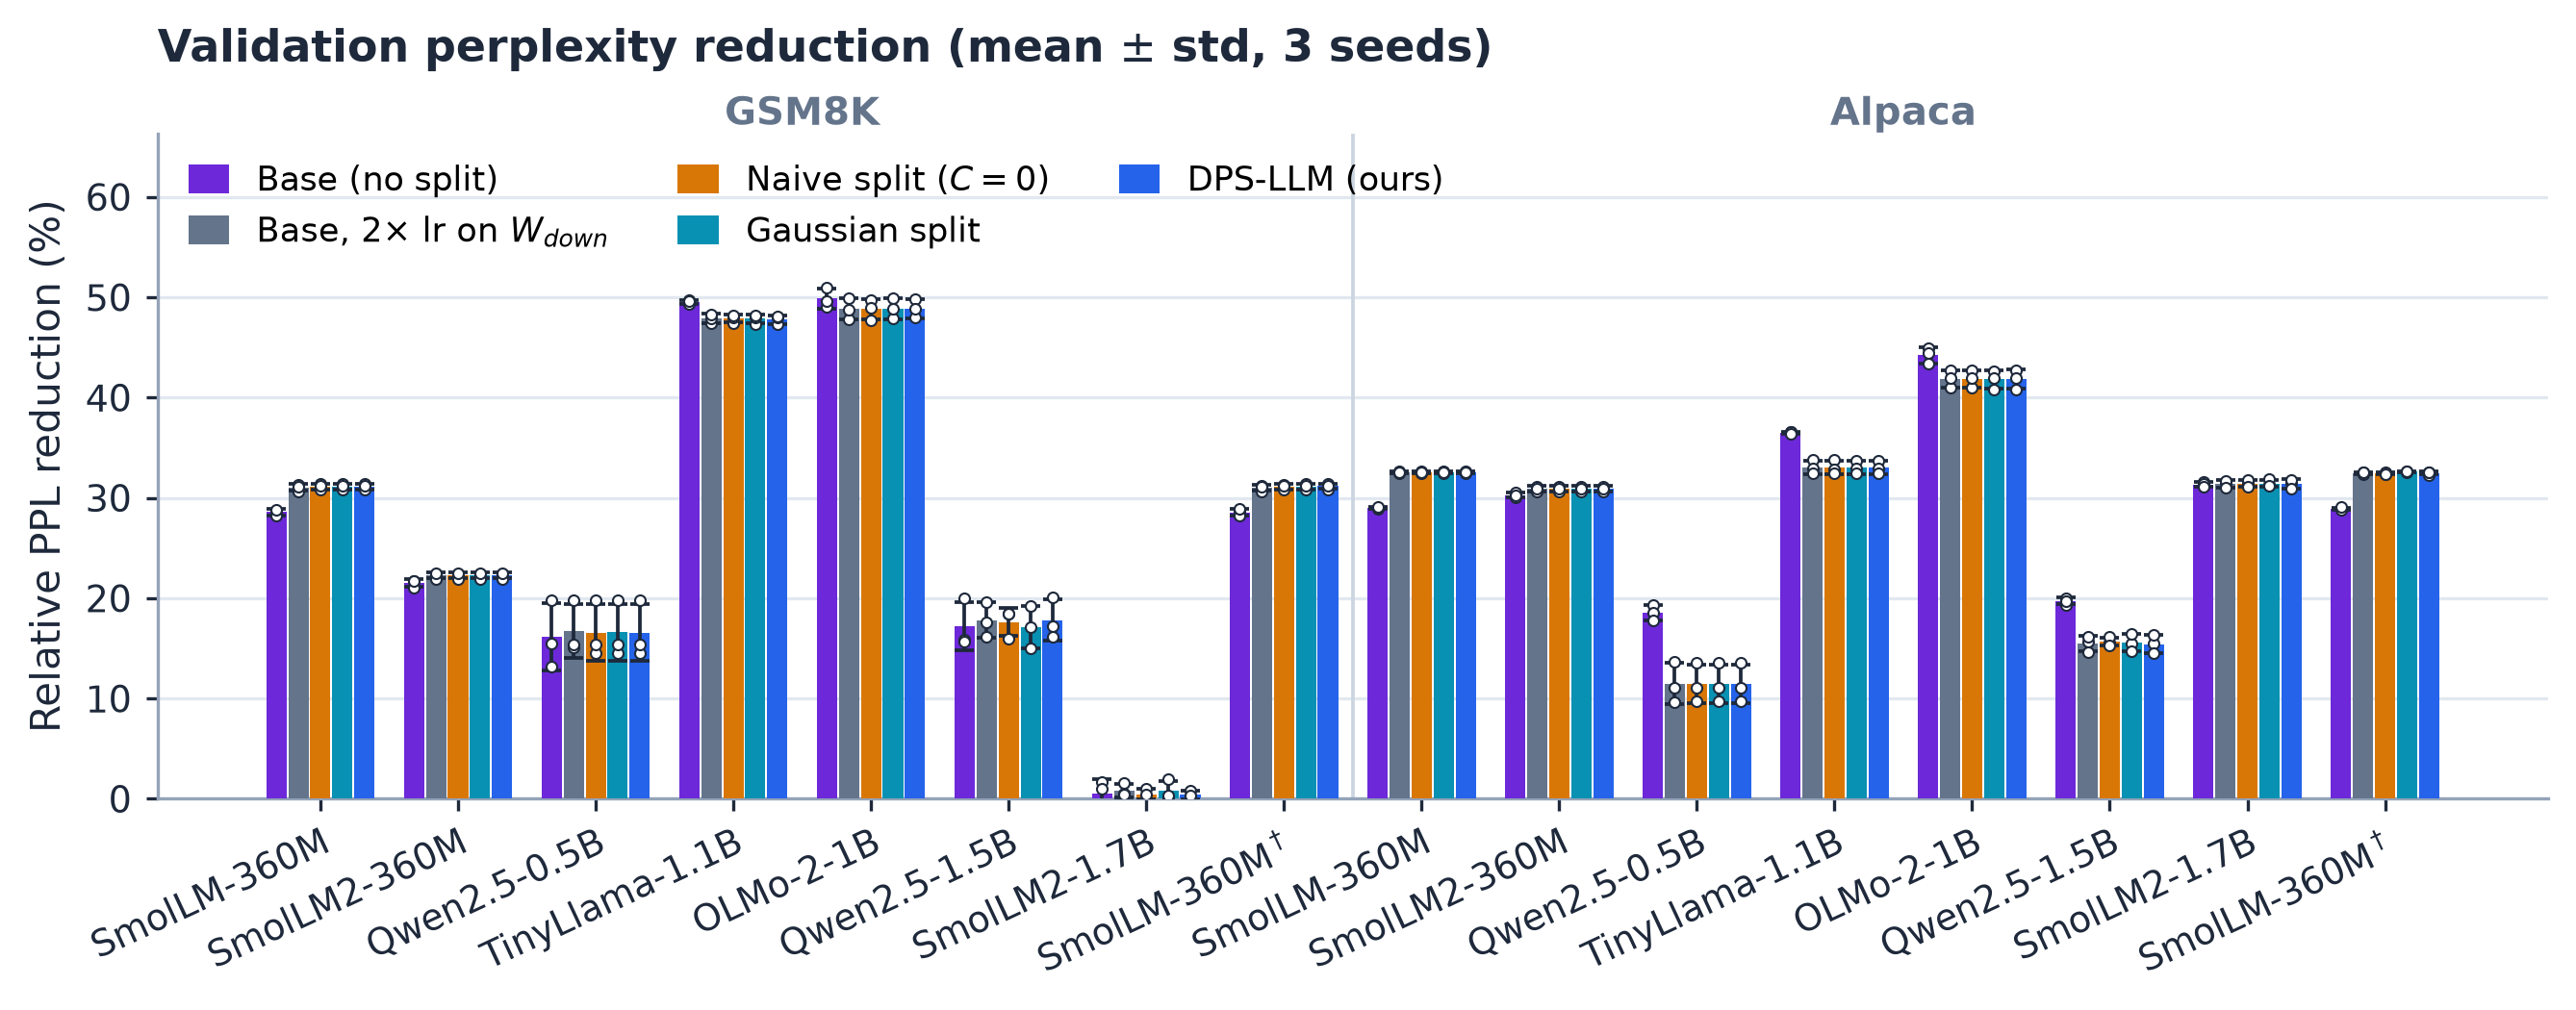
\includegraphics[width=\textwidth]{multi_model_benchmark_comparison.png}
    \caption{\textbf{Benchmark summary}: relative validation-perplexity reduction, mean $\pm$ std over three seeds, with individual seeds as dots. In every setting the three splits (orange, teal, blue) match the matched control (grey), whether they are above or below the unexpanded seed (purple). $^\dagger$: bfloat16 with stochastic rounding.}
    \label{fig:benchmark_results}
\end{figure*}

\subsection{Results}
\label{sec:results}

\paragraph{The split is function-preserving, and the anti-symmetric pairing cancels drift.}
In float32, validation perplexity immediately after the DPS split differs from the seed's by at most $1.3\times10^{-6}$ across all runs, the same as exact duplication ($1.8\times10^{-6}$, from re-associating floating-point sums), whereas Gaussian noise of the same RMS shifts it by up to $2.1\times10^{-4}$. The ablation (Table~\ref{tab:ablation}) shows the same ordering at every noise scale: at $C{=}10^{-1}$ the DPS drift is $1.3\times10^{-3}$ against $1.5\times10^{-2}$ for Gaussian noise, and the anti-symmetric pairing removes the drift that a symmetric $(+\delta,+\delta)$ pairing leaves ($0$ vs.\ $3.0\times10^{-5}$ at $C{=}10^{-4}$), as Proposition~\ref{prop:drift} predicts. Removing the $\tfrac{1}{2}$ factor raises the initial perplexity from 5.13 to 14.47. Under the bfloat16 protocol the split is rounded to nearest, which alone shifts perplexity by up to 0.02.

\paragraph{A split behaves like a learning-rate change.}
In 15 of 18 settings each of the three splits ends within $0.18$ points of the matched control (Table~\ref{tab:empirical_results}, Figure~\ref{fig:benchmark_results}); the exceptions are three noisy GSM8K settings, Qwen2.5-1.5B, SmolLM2-1.7B and Llama-3.2-1B, where the splits are within $0.68$ points of the control and the seed standard deviation is $0.4$--$2.4$. Only one of eighteen DPS-vs-control comparisons reaches $p<0.05$ (SmolLM-360M/GSM8K, $+0.11$ points). Relative to the unexpanded seed at the shared learning rate, splitting looks helpful where the seed is learning-rate-limited (SmolLM-360M: $+2.6$ on GSM8K, $+3.6$ on Alpaca) and harmful where a larger step on $W_{down}$ overshoots (Qwen2.5-0.5B/Alpaca: $-7.1$; Qwen2.5-1.5B/Alpaca: $-4.3$; TinyLlama: $-1.8$ and $-3.5$; OLMo-2-1B: $-1.0$ and $-2.4$; Llama-3.2-1B: $-5.6$ and $-6.0$). The control moves by the same amounts in every case ($+2.5$, $+3.5$, $-7.1$, $-4.2$, $-1.7$, $-3.4$, $-1.0$, $-2.3$, $-5.6$, $-6.1$), so these differences are the step-size effect of Proposition~\ref{prop:lr}, not capacity.

\paragraph{The perturbation does not break the symmetry.}
In float32 the relative distance between paired neurons after 100 steps equals its value at the split to three significant digits ($5.84\times10^{-5}$ for DPS-LLM and $4.13\times10^{-5}$ for Gaussian noise on SmolLM-360M; Figure~\ref{fig:divergence}a), and exactly zero for naive duplication. Across the ablation the distance scales linearly with $C$ and never grows, and the final perplexity is identical to four significant digits for DPS-LLM at every $C\le10^{-2}$ and for Gaussian noise up to $C{=}10^{-3}$ (Table~\ref{tab:ablation}). This is consistent with Proposition~\ref{prop:lr}: a perturbation of relative size $C$ changes the two copies' gradients by $O(C)$, so Adam, whose update depends on the gradient's direction rather than its scale, moves both copies by almost the same step and the initial gap is preserved rather than amplified. Under the bfloat16 protocol, stochastic rounding of each update pulls the copies apart by itself, so even naive duplication reaches a distance of $3.6\times10^{-3}$ on SmolLM-360M (Figure~\ref{fig:divergence}b) and $5$--$12\times10^{-3}$, 64--89\% of the DPS-LLM distance, on the five models of 1B parameters and more; this still yields no consistent gain. Of the fifty-four pairwise comparisons among the three splits only one reaches $p<0.05$ (Gaussian over naive on SmolLM-360M$^\dagger$/Alpaca, $+0.21$ points), fewer than the 2.7 expected by chance.

\paragraph{At matched learning rates the larger model does not win.}
Table~\ref{tab:lr} compares each model's best learning rate for the seed and for DPS-LLM. The differences range from $-3.11$ to $+2.61$ points; the seed is ahead on six of nine settings. The two largest differences come from the largest models. On Qwen2.5-1.5B, DPS-LLM peaks at a lower rate than the seed and diverges at $10^{-4}$ ($-15.6\%$ against $+3.6\%$ for the seed), and on Llama-3.2-1B it degrades much faster than the seed at high rates ($-50.2\%$ against $-15.8\%$ at $10^{-4}$), as expected if the split doubles the effective step on $W_{down}$; on SmolLM2-1.7B both peak at the largest rate swept, so the sweep does not bracket its optimum. Within this budget, the 54--75\% of added parameters do not translate into a consistently lower perplexity.

\paragraph{Accuracy.}
GSM8K exact match on 50 problems is a coarse measure (Table~\ref{tab:accuracy}), but it shows the same pattern. Fine-tuning on reference solutions lowers the accuracy of Qwen2.5-0.5B from 22\% to 9.3\% for the seed and 4.7--5.3\% for the splits and the control, of OLMo-2-1B from 54\% to 16.0\% and 6.7--8.7\%, and of Llama-3.2-1B from 12\% to 3.3\% and 2.7--6.0\%. In all three, the splits stay within 2.6 points (fewer than two problems) of the control, consistent with a larger effective step on $W_{down}$ rather than with the split. The two largest models instead improve: Qwen2.5-1.5B from 12\% to 14.0--17.3\% and SmolLM2-1.7B from 14\% to 32.0--34.0\%, the latter while its GSM8K perplexity falls by less than 1\%, which suggests it mainly learns the answer format; in both, all five conditions lie within 3.3 points, fewer than two of the 50 problems.

\paragraph{Pilot in pure bfloat16.}
With round-to-nearest bfloat16, the $C{=}10^{-4}$ perturbation is absorbed by rounding: the two copies of every neuron kept a cosine similarity of $1.0000$ for 200 steps, and DPS-LLM, Gaussian noise and duplication were statistically indistinguishable ($p\ge0.09$). An emulation of bfloat16 rounding on $\mathcal{N}(0,0.02^2)$ weights shows why: at $C{=}10^{-4}$ the copies differ in only 0.6\% of entries, against 42\% at $C{=}10^{-2}$. The same run also lost most small updates, since an update of $2\times10^{-5}$ is below half a bfloat16 ulp for most weights; SmolLM-360M's base model improved perplexity by 5.3\% in that run despite twice as many steps, against 28.6\% in float32 here.

\begin{figure}[t]
    \centering
    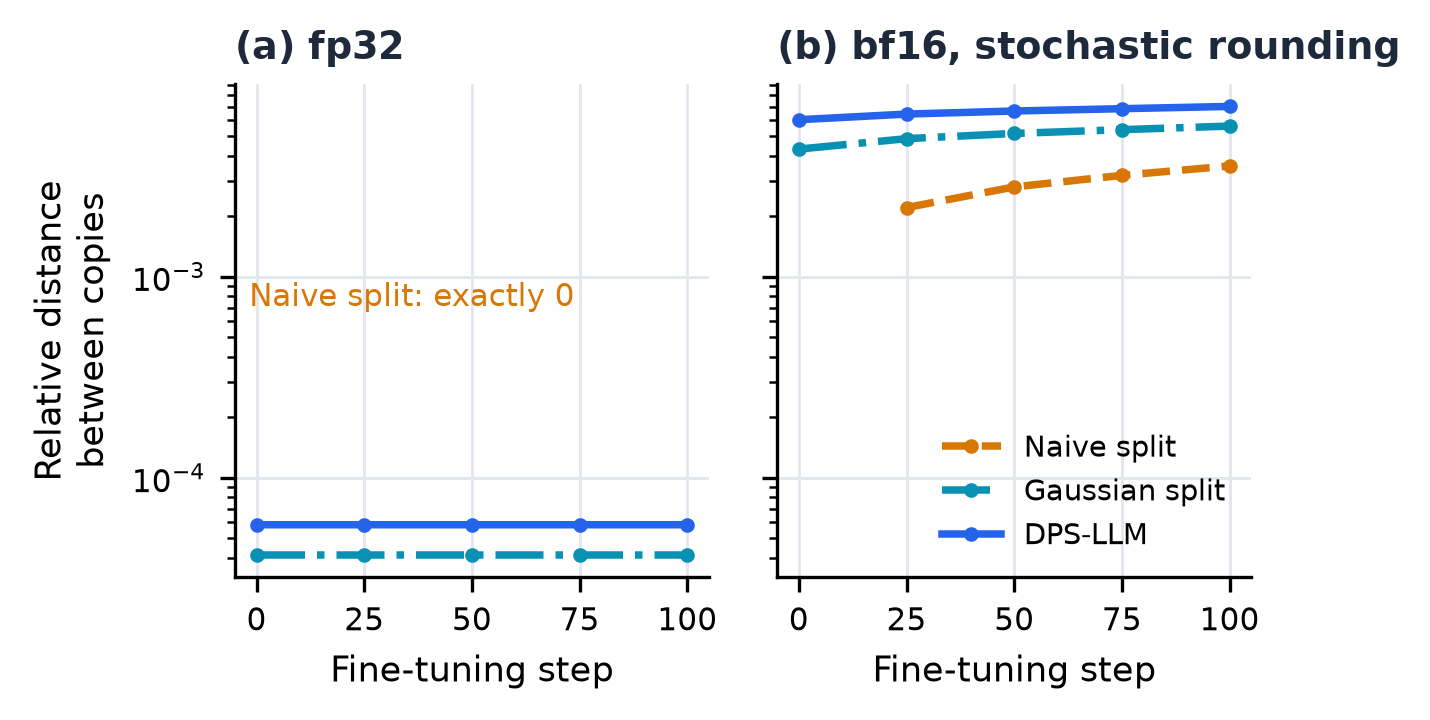
\includegraphics[width=\figwidth]{pair_divergence.png}
    \caption{\textbf{Distance between the two copies of each split neuron} during fine-tuning of SmolLM-360M, mean over seeds and datasets. In float32 (a) the gap created by the perturbation is preserved but never grows. Under bfloat16 with stochastic rounding (b) the rounding itself separates the copies, including for exact duplication.}
    \label{fig:divergence}
\end{figure}

\begin{table}[t]
\centering
\footnotesize
\setlength{\tabcolsep}{4pt}
\caption{\textbf{Best learning rate per model} (GSM8K, seed 42; sweep over $\{1,2,5,10\}\times10^{-5}$): relative perplexity reduction (\%) of the seed and of DPS-LLM, each at its own best rate.}
\label{tab:lr}
\begin{adjustbox}{max width=\columnwidth}\begin{tabular}{@{}lccccc@{}}
\toprule
\textbf{Model} & \multicolumn{2}{c}{\textbf{Base}} & \multicolumn{2}{c}{\textbf{DPS-LLM}} & $\Delta$ \\
\cmidrule(lr){2-3}\cmidrule(lr){4-5}
 & lr & red. & lr & red. & \\
\midrule
SmolLM-360M & $10^{-4}$ & 34.40 & $10^{-4}$ & 34.54 & +0.14 \\
SmolLM2-360M & $5{\times}10^{-5}$ & 23.04 & $5{\times}10^{-5}$ & 22.83 & $-$0.20 \\
Qwen2.5-0.5B & $2{\times}10^{-5}$ & 15.45 & $10^{-5}$ & 15.07 & $-$0.38 \\
TinyLlama-1.1B$^\dagger$ & $10^{-5}$ & 51.45 & $10^{-5}$ & 50.59 & $-$0.87 \\
Llama-3.2-1B$^\dagger$ & $10^{-5}$ & 36.28 & $10^{-5}$ & 34.98 & $-$1.30 \\
OLMo-2-1B$^\dagger$ & $10^{-5}$ & 52.04 & $10^{-5}$ & 51.83 & $-$0.21 \\
Qwen2.5-1.5B$^\dagger$ & $5{\times}10^{-5}$ & 20.60 & $10^{-5}$ & 17.49 & $-$3.11 \\
SmolLM2-1.7B$^\dagger$ & $10^{-4}$ & 7.37 & $10^{-4}$ & 9.98 & +2.61 \\
SmolLM-360M$^\dagger$ & $10^{-4}$ & 34.37 & $10^{-4}$ & 34.57 & +0.19 \\
\bottomrule
\end{tabular}
\end{adjustbox}
\end{table}

\begin{table}[t]
\centering
\footnotesize
\setlength{\tabcolsep}{4pt}
\caption{\textbf{GSM8K exact-match accuracy (\%)} on 50 test problems before fine-tuning and after it (mean over seeds).}
\label{tab:accuracy}
\begin{adjustbox}{max width=\columnwidth}\begin{tabular}{@{}lcccccc@{}}
\toprule
\textbf{Model} & \textbf{Before} & \textbf{Base} & \textbf{2$\times$ ctrl} & \textbf{Naive} & \textbf{Gauss.} & \textbf{DPS} \\
\midrule
SmolLM-360M & 2 & 0.7 & 3.3 & 4.0 & 4.0 & 4.0 \\
SmolLM2-360M & 0 & 5.3 & 7.3 & 8.0 & 7.3 & 8.0 \\
Qwen2.5-0.5B & 22 & 9.3 & 5.3 & 4.7 & 4.7 & 4.7 \\
TinyLlama-1.1B$^\dagger$ & 0 & 2.0 & 2.7 & 2.0 & 4.0 & 0.7 \\
OLMo-2-1B$^\dagger$ & 54 & 16.0 & 7.3 & 8.7 & 6.7 & 7.3 \\
SmolLM-360M$^\dagger$ & 2 & 2.7 & 2.0 & 3.3 & 2.0 & 2.0 \\
\bottomrule
\end{tabular}
\end{adjustbox}
\end{table}

\begin{table}[t]
\centering
\footnotesize
\setlength{\tabcolsep}{3pt}
\caption{\textbf{Ablations} on SmolLM-360M/GSM8K, float32, seed 42, 50 steps. \emph{Init drift}: change of validation perplexity caused by the split (base: 5.13). \emph{Red.}: relative perplexity reduction after fine-tuning. \emph{Pair dist.}: relative distance between paired neurons after fine-tuning.}
\label{tab:ablation}
\begin{adjustbox}{max width=\columnwidth}\begin{tabular}{@{}lccc@{}}
\toprule
\textbf{Variant} & \textbf{Init drift} & \textbf{Red.\ (\%)} & \textbf{Pair dist.} \\
\midrule
Base (no split) & 0 & 22.31 & -- \\
Naive split & 0 & 25.78 & 0 \\
\midrule
DPS, $C{=}10^{-5}$ & 0 & 25.78 & $5.8{\times}10^{-6}$ \\
Gaussian, $C{=}10^{-5}$ & $+6.2{\times}10^{-7}$ & 25.78 & $4.1{\times}10^{-6}$ \\
DPS, $C{=}10^{-4}$ & 0 & 25.78 & $5.8{\times}10^{-5}$ \\
Gaussian, $C{=}10^{-4}$ & $+3.2{\times}10^{-6}$ & 25.78 & $4.1{\times}10^{-5}$ \\
DPS, $C{=}10^{-3}$ & $+5.1{\times}10^{-7}$ & 25.78 & $5.8{\times}10^{-4}$ \\
Gaussian, $C{=}10^{-3}$ & $+2.5{\times}10^{-5}$ & 25.78 & $4.1{\times}10^{-4}$ \\
DPS, $C{=}10^{-2}$ & $+1.4{\times}10^{-5}$ & 25.78 & $5.8{\times}10^{-3}$ \\
Gaussian, $C{=}10^{-2}$ & $+3.5{\times}10^{-4}$ & 25.75 & $4.1{\times}10^{-3}$ \\
DPS, $C{=}10^{-1}$ & $+1.3{\times}10^{-3}$ & 25.80 & $5.8{\times}10^{-2}$ \\
Gaussian, $C{=}10^{-1}$ & $+1.5{\times}10^{-2}$ & 25.55 & $4.1{\times}10^{-2}$ \\
\midrule
DPS, symmetric $(+\delta,+\delta)$ & $+3.0{\times}10^{-5}$ & 25.78 & 0 \\
DPS, no $\tfrac{1}{2}$ factor & +9.34 & 60.52 & $5.8{\times}10^{-5}$ \\
\bottomrule
\end{tabular}
\end{adjustbox}
\end{table}

% -----------------------------------------------------------------------------
\section{Conclusion}
The function-preserving half of DPS-LLM works as designed: placing the factor $\tfrac{1}{2}$ on the down projection grows the SwiGLU blocks of a pre-trained LLM without changing its output, and the anti-symmetric, polarity-signed perturbation cancels first-order drift in practice, by two orders of magnitude relative to Gaussian noise. The symmetry-breaking half does not take effect during fine-tuning: the gap between paired neurons is preserved but never amplified, so the split model behaves like its seed, and under Adam that means like its seed with a doubled learning rate on $W_{down}$. A matched control reproduces every gain and loss we observe, and at each model's best learning rate the split model is not consistently better than the seed. We draw two lessons for work on model growth. Comparisons of a grown model with its seed at a shared learning rate conflate capacity with step size and need the matched control; and symmetry breaking should be verified by measuring whether the copies diverge, not assumed from the perturbation. Whether larger noise, longer training from scratch-scale budgets, or growth during pre-training changes this picture remains open; the same operator applies to MoE upcycling and LoRA rank growth, which we have not evaluated.

% -----------------------------------------------------------------------------
\section*{Limitations}
\textbf{Scale.} We evaluate eight models up to 1.7B parameters, fine-tuned for 50 optimiser updates on 256 examples; capacity effects may only appear with larger models, larger datasets or longer training, and in pre-training rather than fine-tuning.
\textbf{Statistics.} Three seeds per condition detect only differences of a few tenths of a point; the learning-rate sweep and the ablations use a single seed, and the sweep does not bracket the best rate of SmolLM2-1.7B.
\textbf{Precision.} The five models of 1B parameters and more use bfloat16 with stochastic rounding and a larger noise scale than the float32 models, so their noise condition is not identical; on SmolLM-360M the two protocols agree within $0.2$ points for every condition.
\textbf{Scope.} Only width splitting of the MLP was evaluated, with only the MLP parameters trainable; depth growth, attention-head splitting, the MoE and LoRA regimes, and full-parameter fine-tuning are untested. We measure perplexity and GSM8K exact match but not instruction-following quality for Alpaca-Cleaned.
\textbf{Data provenance.} The Alpaca-Cleaned validation examples come from its training split; they are unseen during our fine-tuning but may have been seen during the checkpoints' original training.

\section*{\ethicsheading}
This work modifies the architecture of publicly released language models and uses two public datasets (GSM8K, MIT licence; Alpaca-Cleaned, CC~BY-NC~4.0) and eight public checkpoints (Qwen2.5-0.5B-Instruct, Qwen2.5-1.5B-Instruct, SmolLM-360M-Instruct, SmolLM2-360M-Instruct, SmolLM2-1.7B-Instruct, TinyLlama-1.1B-Chat and OLMo-2-0425-1B-Instruct, all Apache~2.0; Llama-3.2-1B-Instruct, Llama~3.2 Community License, used under its terms for research). Growing a model does not change the biases or safety properties of its seed, and a grown model inherits any limitations of the original checkpoint; practitioners should re-run their safety evaluations after expansion. All experiments ran on a free cloud GPU tier with a small compute footprint (about 23 hours on a two-T4 instance for the benchmark, sweeps and ablations, and 4 for the pilot). No human subjects or personal data were involved.

\ifdefined\FINAL\def\showacknowledgements{}\fi
\ifdefined\ARXIV\def\showacknowledgements{}\fi
\ifdefined\showacknowledgements
\section*{Acknowledgements}
The author thanks Dr.~M.~Ali Tahir (SEECS, National University of Sciences and Technology) for supervising the thesis on which this work builds.
\fi


\bibliography{references}
\bibliographystyle{plainnat}

\appendix
% Appendix of the paper, shared by all venue versions (see body.tex).

\section{Additional Growth Regimes}
\label{app:regimes}
The same rows/columns operator and anti-symmetric noise apply to two further situations. Both are implemented in the released code but were not part of the benchmark in Section~\ref{sec:setup}.

\paragraph{Dense-to-MoE upcycling.}
A dense SwiGLU block is cloned into $E$ experts with independent calculated-noise draws $\Delta^{(e)}$ and combined by a top-$k$ softmax router \citep{shazeer2017outrageously,fedus2022switch}:
\begin{align}
    \mathrm{Expert}_e(x) &= \mathrm{SwiGLU}\big(x;\,W+\Delta^{(e)}\big), \\
    g(x) &= \mathrm{Top}\text{-}k\big(\mathrm{softmax}(W_r x)\big).
\end{align} With $k=E$ and a uniform router the layer is initially function-preserving; the perturbations give each expert a distinct gradient trajectory from the first step, which is the failure mode that sparse upcycling \citep{komatsuzaki2022sparse} must otherwise wait for the router to resolve.

\paragraph{LoRA rank doubling.}
For a LoRA adapter $\Delta W = BA$ with $A\in\mathbb{R}^{r\times d_{in}}$, $B\in\mathbb{R}^{d_{out}\times r}$ \citep{hu2021lora}, the rank is grown $r\to2r$ by
\begin{equation}
    A' = \begin{bmatrix} A \\ A+\Delta_A \end{bmatrix}, \qquad
    B' = \begin{bmatrix} B & \Delta_B \end{bmatrix},
\end{equation}
where $\Delta_B$ is calculated noise on a zero matrix, i.e.\ near zero. Because the new columns of $B$ are (near) zero, $B'A' = BA + \Delta_B(A+\Delta_A)\approx BA$, so the adapted function is preserved while the optimiser gains $r$ additional rank-one directions.

\section{Prompt Templates}
\label{app:prompts}
Each example is rendered as plain text and tokenised with the checkpoint's own tokeniser; no chat template is applied.
\begin{center}\small
\begin{tabular}{@{}l>{\ttfamily}p{0.7\columnwidth}@{}}
\toprule
\textbf{Dataset} & \textrm{\textbf{Template}} \\
\midrule
GSM8K & Question: \{question\}\textbackslash n Answer: \{answer\} \\
Alpaca & Instruction: \{instruction\}\textbackslash n [Input: \{input\}\textbackslash n] Response: \{output\} \\
\bottomrule
\end{tabular}
\end{center}
The bracketed \texttt{Input} line is emitted only when the example has a non-empty input field.

\section{Reproducibility}
\label{app:repro}
The split operator (\texttt{split\_huggingface\_llm.py}), the synthetic experiment behind Figure~\ref{fig:training_curve}, the Kaggle notebooks that produced every table and figure, the scripts that generate them from the raw results, and every per-seed result, loss history and neuron-pair distance trace are available at \repourl. The benchmark notebook runs on a free Kaggle session with two T4 GPUs; the float32 models take about 0.8 hours each and TinyLlama 2.4 hours for 30 runs, and no run starts after 11 hours, so a session always saves its checkpointed results.


\end{document}
